\documentclass[abstracton,12pt]{scrartcl}
    
\usepackage[utf8]{inputenc}
% \usepackage[T1]{fontenc}
\usepackage[dvipsnames]{xcolor}
\usepackage{fancyhdr}
\usepackage{graphicx}
\usepackage{tikz}
\usepackage{listings}
\usepackage{amssymb}
\usepackage{amsfonts}
\usepackage{amsmath}
\usepackage{amsthm}
\usepackage{pdfpages}
\usepackage{forest}
\usepackage{multicol}
\usepackage{varwidth}
\usepackage{verbatim}
\usepackage{minted}
\usepackage{framed}
\usepackage[ruled,vlined]{algorithm2e}
\usepackage{caption}
\usepackage{subcaption}
\usepackage{cleveref}
\usepackage{soul}
\usepackage{float}
\usepackage{wrapfig}
\usepackage{lipsum}
% \usepackage{geometry}
% \usepackage{titlesec}

% \forestset{qtree/.style={for tree={parent anchor=south, child anchor=north,align=left,inner sep=0pt}}}
\graphicspath{
  {images/},
  {images/unproductive_nodes/},
  {images/volatility_threshold/},
  {images/sliding_window/},
  {images/gc/},
  {images/skew/},
  {images/updates_per_query/},
  {images/qtp_cost/},
  {images/cdf/},
  {images/period_runtime/},
  {images/periodicity/}
}

% \setlength{\multicolsep}{6.0pt plus 2.0pt minus 1.5pt}% 50% of original values
% \titleformat{\chapter}{}{\thechapter}{}{}
% \titlespacing{\chapter}{-100pt}{-100pt}{-100pt}

% --------- 

\titlehead{Department of Informatics, University of Zürich}
\subject{\vspace*{2cm}BSc Thesis}
\title{An Adaptive Index for Hierarchical Database Systems}
\author{
    Rafael Kallis\\[-5pt]
    \scriptsize Matrikelnummer: 14-708-887\\[-5pt]
    \scriptsize Email: \texttt{rk@rafaelkallis.com}
}
\date{\vspace*{2cm}February 1, 2018}
\publishers{
    \small supervised by Prof.\ Dr.\ Michael\ Böhlen and Kevin\ Wellenzohn \\[5cm]
    \begin{tikzpicture}[overlay]
    \node at (-3,-3) {
\includegraphics[height=1.5cm]{IFIlogo}};
    \node at (7,-3) {
\includegraphics[height=1.5cm]{dbtgBW}};
    \end{tikzpicture}
}

% \dedication{dedicated to xxx}

% --------- 

\theoremstyle{definition}

\newtheorem{definition}{Definition}
% \newtheorem{figure}{Figure}
\newtheorem{example}{Example}
% \newtheorem{theorem}{Theorem}
% \newtheorem{lemma}{Lemma}

\crefname{algocfline}{algorithm}{algorithms}
\Crefname{algocfline}{Algorithm}{Algorithms}

\crefname{figure}{Fig.}{Figs.}
\Crefname{figure}{Figure}{Figures}

\crefname{example}{Ex.}{Ex.}
\Crefname{example}{Example}{Examples}

% \newenvironment{proof}
%     {\noindent{\bf Proof:\rm}}{\hfill$\Box$\vspace{\medskipamount}}


% \def\bbbr{{\rm I\!R}}
% \def\bbbm{{\rm I\!M}}
% \def\bbbn{{\rm I\!N}}
% \def\bbbz{{\rm I\!Z}}

\definecolor{shadecolor}{rgb}{0.97,0.97,0.97}
\usetikzlibrary{decorations.pathreplacing}

\definecolor{C0}{RGB}{31,119,180}
\definecolor{C1}{RGB}{255,127,14}
\definecolor{C2}{RGB}{44,192,44}
\definecolor{C3}{RGB}{214,39,40}
\definecolor{C4}{RGB}{148,103,189}

\begin{document}

\maketitle
\thispagestyle{empty}
% \chapter*{Acknowledgements}

% \newpage\null\thispagestyle{empty}\newpage

\newpage
\thispagestyle{empty}
\vspace*{7cm}

\section*{Abstract}

The workload aware property index is a hierarchical index which adapts to the
database's recent transactional workload by not pruning volatile index nodes,
that is nodes which are frequently inserted or deleted, in order to increase
update performance. When the workload changes, these nodes cease to be volatile
and become unproductive if they and their descendants, neither contribute to a
query match, nor are volatile.

Unproductive nodes in hierarchical indexes waste space and slow down queries.
We propose periodic Garbage Collection and Query-Time Pruning in order to
clean unproductive nodes in the index. We implement the techniques in Apache
Jackrabbit Oak and
provide an extensive experimental evaluation to stress test the algorithms and
show that the database throughput increases considerably when periodic Garbage
Collection or Query-Time Pruning are applied.

\newpage
\thispagestyle{empty}
\vspace*{7cm}

\section*{Zusammenfassung}

Der ``workload aware property index'' ist ein hierarchischer Index, der sich an
die jüngste Transaktionslast der Datenbank anpasst, indem er volatile
Indexknoten, dh Knoten, die häufig eingefügt oder gelöscht werden, nicht löscht,
um die Schreibleistung zu erhöhen. Wenn sich die Arbeitslast ändert, sind
diese Knoten nicht mehr volatil und werden unproduktiv, wenn sie und ihre
Nachkommen weder zu einer Abfrage beitragen noch volatil sind.

Unproduktive Knoten in hierarchischen Indizes verschwenden Speicherplatz und
verlangsamen die Abfragen. Wir schlagen periodische Indexreinigung
und Abfragezeitbe- reinigung vor, um den Index von unproduktiven Knoten zu
bereinigen. Wir implementieren
unsere Techniken in Apache Jackrabbit Oak und bieten eine umfangreiche
experimentelle Auswertung um die Algorithmen unter hoher Last zu testen und
zeigen, dass der Datenbankdurchsatz erheblich zunimmt, wenn periodische
Indexreinigung oder Abfragezeitbereinigung benutzt wird.

\newpage
\thispagestyle{empty}

\tableofcontents

\newpage
\thispagestyle{empty}

\listoffigures

\newpage
% \listoftables

\newpage\null\thispagestyle{empty}\newpage

\section{Introduction}

Frequently adding and removing data from hierarchical indexes causes them to
repeatedly grow and shrink. A single insertion or deletion can trigger a
sequence of structural index modifications (node insertions/deletions) in a
hierarchical index. Skewed and update-heavy workloads trigger repeated
structural index updates over a small subset of nodes to the index.
Informally, a frequently added or removed node is called \textit{volatile}.
Volatile nodes decrease index update performance due to two reasons. First,
frequent structural index modifications are expensive since they cause many disk
accesses. Second, frequent structural index modifications also increase the
likelihood of conflicting index updates by concurrent transactions. Conflicting
index updates further decrease update performance since concurrency control
protocols need to resolve the conflict.

Wellenzohn et al.~\cite{KW17} propose the Workload-Aware Property Index (WAPI).
The WAPI exploits the workload's skewness by identifying and not removing
volatile nodes from the index, thus significantly reducing the number of
expensive structural index modifications. Since fewer nodes are
inserted/deleted, the likelihood of conflicting index updates by concurrent
transactions is reduced.

Some Content Management Systems (CMS) make use of hierarchical databases. The Adobe
Experience
Manager,\footnote{http://www.adobe.com/marketing-cloud/experience-manager.html}
Adobe's enterprise CMS, works with the hierarchical database system Apache
Jackrabbit Oak (Oak). CMSs yield skewed, update-heavy and changing
workloads. They frequently update a small changing subset of index nodes. Such
workloads decrease WAPI's query performance.

When the workload characteristics change, new index nodes can become volatile
while others cease to be volatile and become \textit{unproductive}. Unproductive
index nodes slow down queries, as traversing an unproductive node is useless
because unproductive nodes do not contain any data 
and thus cannot yield a query match. Additionally, unproductive nodes
occupy storage space that could otherwise be reclaimed. lf the workload changes
frequently, unproductive nodes accumulate in the index and the query
performance deteriorates over time. Therefore, unproductive nodes must be
cleaned to keep query performance stable over time and reclaim disk space as
the workload changes.

Wellenzohn et al.~\cite{KW17} propose periodic Garbage Collection (GC), which
traverses the entire index subtree and prunes all unproductive index nodes at
once. Additionally we propose Query-Time Pruning (QTP), an incremental approach
to cleaning unproductive nodes in the index. The idea is to turn queries into
updates. Since Oak already traverses unproductive nodes as part of query
processing, these nodes could be pruned at the same time. 
With QTP, only one query has to traverse an unproductive node, while subsequent
queries can skip this overhead and thus perform better.
The goal of this BSc thesis is to study, implement and empirically compare GC
and QTP as proposed by \cite{KW17} in the open-source hierarchical 
database Apache Jackrabbit Oak.

\newpage\null\thispagestyle{empty}\newpage

\section{Background}

% \subsection{Apache Jackrabbit Oak (Oak)}

% Oak is a hierarchical distributed database system which uses a
% hierarchical index for efficient query processing. Multiple transactions can
% work concurrently by making use of
% Multiversion Concurrency Control (MVCC)~\cite{GW02}, a commonly used optimistic
% concurrency control technique~\cite{TM11}.

% \Cref{fig:architecture} depicts Oak's data-sharing architecture. Oak embodies the
% \textit{Database Tier}. Multiple Oak instances can operate concurrently.
% Whilst Oak is responsible for handling the database logic, it stores the actual
% data on MongoDB,\footnote{https://www.mongodb.com/what-is-mongodb} labeled as
% \textit{Persistence Tier}. On the other end, applications can make use of Oak as
% shown in \Cref{fig:architecture} under \textit{Application Tier}.
% One such application is Adobe's enterprise content management system (CMS),
% the Adobe Experience
% Manager.

% \begin{figure}[h]
%   \centering
%   \begin{tikzpicture}[scale=0.8,thick]
%     \node (mongo) at (0, 0) {
\includegraphics[width = 0.7cm]{MONGO}}; \node
%     (oak_a) at (-2, 2) {
\includegraphics[width = 0.7cm]{OAK}}; \node (oak_b)
%     at (0, 2) {
\includegraphics[width = 0.7cm]{OAK}}; \node (oak_c) at (2, 2)
%     {
\includegraphics[width = 0.7cm]{OAK}}; \node (app_a) at (-2, 4)
%     {
\includegraphics[width = 0.7cm]{AEM}}; \node (app_b) at (0, 4)
%     {
\includegraphics[width = 0.7cm]{AEM}}; \node (app_c) at (2, 4)
%     {
\includegraphics[width = 0.7cm]{AEM}}; \node (mongo_desc) at (5, 0)
%     {\footnotesize \textit{Persistence Tier}}; \node (oak_desc) at (5, 2)
%     {\footnotesize \textit{Database Tier}}; \node (mongo_desc) at (5, 4)
%     {\footnotesize \textit{Application Tier}}; \foreach \from/\to in
%     {app_a/oak_a, app_b/oak_b, app_c/oak_c, oak_a/mongo, oak_b/mongo,
%       oak_c/mongo} \draw [->] (\from) -- (\to);
%   \end{tikzpicture}
%   \caption{Oak's system architecture}
%   \label{fig:architecture}
% \end{figure}

\subsection{CMS Workload}

\label{sec:application_scenario}

Depending on the data model, applications might use a hierarchical database
system such as Apache Jackrabbit Oak, called Oak. A content management system
(CMS) might choose Oak because
the database reflects the hierarchical structure of a webpage.
Content management systems have specific workloads.
These workloads have distinct properties: they are \textit{skewed},
\textit{update-heavy} and \textit{changing}~\cite{KW17}. CMSs frequently use a
job-queuing system that has the noted characteristics.

Consider a social media feed as a running example. Only a few posts are popular.
These posts have many comments or likes. Since most of the interactions
(comments, likes) are on a small subset of the posts, we have a skewed workload.
Users submit new posts or interact with existing posts by
writing comments for example, creating an update-heavy workload. As time
passes, new posts are created. Users are more likely to interact with recent
posts than older ones, hence the workload changes over time.

When a user submits a new post, a job is sent to the CMS for processing. % If the
% post has an image, the CMS needs to compress the image and
% create a thumbnail. A job is created for processing the uploaded image.
A background thread is periodically checking for pending
jobs. A pending job is signaled using node properties in Oak.
The CMS adds a property to the respective node in
order to signal the background thread that the specific node has a pending job requiring
processing. A node's ``pub'' property signals when the job has to be processed.
Setting the value of ``pub'' to ``now'' indicates that the job must be processed
immediately.
Once the background thread detects the node, the job is processed and the ``pub''
property is removed.

From now on, we shall refer to a workload with the properties mentioned above as
a \textit{CMS workload}. When a hierarchical database operates under a CMS
workload, we can increase its update performance using the workload aware
property index.

\subsection{Workload Aware Property Index (WAPI)}
\label{sec:wapi}

Oak mostly executes content-and-structure (CAS) queries~\cite{CM15}.
We denote node $n$'s property $k$ as $n[k]$ and node $n$'s descendants as
$desc(n)$.

\begin{definition}[CAS Query]
  Given node $m$, property $k$ and value $v$, a CAS query
  $Q(k,v,m)$ returns all descendants of $m$ which have $k$ set to $v$, i.e.,
  $$ Q(k,v,m) = \{ n | n \in desc(m) \land n[k] = v\} $$
  \label{def:cas-query}
\end{definition}

\begin{example}[CAS Query]
  Consider \Cref{fig:hierarchical_db}. CAS-Query $Q(\text{pub},\text{now},\texttt{/a})$,
  which queries for every descendant of \texttt{/a} with
  ``pub'' set to ``now'', would evaluate to $Q(\text{pub},\text{now},\texttt{/a}) = \{\texttt{/a/b/d}\}$,
  since \texttt{/a/b/d} is the only descendant of \texttt{/a} with ``pub'' set
  to ``now''.
  \label{ex:cas_query}
\end{example}

\Cref{fig:hierarchical_db} depicts a database instance with the workload aware
property index (WAPI).
The WAPI is a hierarchical index which indexes the properties of nodes in order
to answer CAS queries efficiently.
The WAPI is hierarchically organized under node \texttt{/i}, the
\textit{Index Subtree Root}.
The second level consists of all properties $k$ we want
to index, such as ``pub''.
The third level contains any values $v$ of property $k$, for example
``now''.
The remaining levels replicate all nodes from the root node to any
content node with $k$ set to $v$.

When processing a CAS query, Oak traverses the WAPI in order to answer the query
efficiently. Any index node has a \textit{corresponding} content node.
Given index node $n$, we denote $n$'s corresponding content node as $*n$.
If index node $n$'s path is $path(n) = \texttt{/i/k/v/m} = \texttt{/i/k/v/}\lambda_1\texttt{/}\dots\texttt{/}\lambda_d$, then $n$'s corresponding content
node $*n$ has the path $path(*n) = \texttt{m} = \texttt{/}\lambda_1\texttt{/}\dots\texttt{/}\lambda_d$.

\begin{figure}[h]
  \centering
  \footnotesize
  \begin{forest}
    [
    [$\lambda:i$
    [$\lambda:\text{pub}$
    [$\lambda:\text{now}$
    [$\lambda:a$
    [$\lambda:b$
    [$\lambda:d$ \\ $\text{pub}:\text{now}$, align=center, base=bottom, name=i_node] {
      \draw[<-,gray] (.north west)--++(-5em,1em)
      node[anchor=east]{\textit{Matching Node}};
    }
    ]
    [,phantom]
    ]
    ]
    ]
    ] {
      \draw[<-,gray] (.south west)--++(-5em, -1em)
      node[anchor=east]{\textit{Index Subtree Root}};
    }
    [$\lambda:a$
    [$\lambda:b$
    [$\lambda:d$ \\ $\text{pub}:\text{now}$, align=center, base=bottom, name=c_node]
    ]
    [$\lambda:c$
    [$\lambda:e$]
    ]
    ] {
      \draw[<-,gray] (.south east)--++(5em, -1em)
      node[anchor=west]{\textit{Content Subtree Root}};
    }
    ]
    \draw[->,dotted] (i_node) to[out=east, in=south] node[gray,midway,right]{\textit{corresponding content node}} (c_node);
  \end{forest}
  \caption[An instance of a hierarchical database]{An instance of a
    hierarchical database. The index subtree is rooted
    at \texttt{/i}. The content subtree is rooted at \texttt{/a}. Index node
    \texttt{/i/pub/now/a/b/d} is matching, since its corresponding content node,
    \texttt{/a/b/d}, has property ``pub'' set to ``now''.}
  \label{fig:hierarchical_db}
\end{figure}

\begin{definition}[Matching Node]
  Index node $n$, with path \texttt{/i/k/v/m}, is matching
  iff $n$ and $n$'s corresponding content node $*n$, with path \texttt{m}, have property
  \texttt{k} set to \texttt{v}, i.e.,
  $$ matching(n) \iff *n[k] = v \land n[k] = v $$
  \label{def:matching_node}
\end{definition}

\begin{example}[Matching Node]
  Consider \Cref{fig:hierarchical_db}. The subtree rooted at \texttt{/a} is
  the content subtree. The subtree rooted at \texttt{/i} is the index
  subtree. Node \texttt{/i/pub/now/a/b/d} is matching, since its corresponding
  content node, \texttt{/a/b/d}, has property ``pub'' set to ``now'' as well as
  \texttt{i/pub/now/a/b/d} itself, too.
\end{example}

From the CMS workload described in \Cref{sec:application_scenario} we can 
infer that the index subtree has a small number of
matching nodes relative to the total number of nodes in the content subtree. The index is
 used to signal pending jobs to the background thread using
the ``pub'' property. Assuming jobs are processed by
the background thread and removed from the index faster than they are created,
the number of matching nodes should be close to zero. We infer that, an index subtree
which resembles a job-queuing system under a CMS workload, should have
almost no matching nodes. 

The CMS workload is also skewed and update-heavy, therefore causing repeated structural index
updates (insertions/deletions) over a small subset of nodes to the index.
The WAPI takes into account if an index node is frequently added and removed,
i.e. \textit{volatile} (see \Cref{def:volatile_node}), before performing structural
index modifications. If a node is considered volatile, we do not remove it from the index.

Volatility is the measure which is used by the WAPI in order to distinguish
whether to remove a node or not from the index.
Wellenzohn et al.~\cite{KW17} propose to look at the recent transactional
workload to check whether a node $n$ is volatile. The workload on Oak instance
$O_i$ is represented by a sequence $H_i = \langle \ldots, G^a, G^b, G^c
\rangle$ of snapshots, called a \textit{history}. A snapshot represents an immutable
committed tree of the database. Let $t_n$ be the current time and
$t(G^b)$ be the point in time snapshot $G^b$ was committed, $N(G^a)$ is the
set of nodes which are members of snapshot $G^a$. We use a superscript $a$
to emphasize that a node $n^a$ belongs to tree $G^a$. $pre(G^b)$ is the
predecessor of snapshot $G^b$ in $H_i$.

Given two snapshots $G^a$ and $G^b$, we write $n^a$ and $n^b$ to emphasize that
nodes $n^a$ and $n^b$ are two versions of the same node $n$, i.e., they have
the same absolute path from the root node.

Node $n$ is volatile iff $n$'s volatility count is at least $\tau$, called
volatility threshold. The volatility count of $n$ is defined as the number of
times $n$ was added or removed from snapshots in a sliding window of length
$L$ over history $H_i$.

\begin{definition}[Volatility Count]
  The volatility count $vol(n)$ of index node $n$ on Oak instance $O_i$, is the number of
  times node $n$ was added or removed from snapshots contained in a Sliding
  Window of Length $L$ over history $H_i$.
  \begin{align*}
    vol(n) = | \{ G^b | G^b \in H_i \land t(G^b) \in [t_n-L+1, t_n] \land \exists G^a[ \\
    \qquad G^a = pre(G^b) \land ([n^a \notin N(G^a) \land n^b \in N(G^b)]\lor \\
    \qquad [n^a \in N(G^a) \land n^b \notin N(G^b)] )]\} |
  \end{align*}
  \label{def:vol_count}
\end{definition}

\vspace{-4mm}

\begin{definition}[Volatile Node]
  Index node $n$ is volatile iff $n$'s volatility count (see
  \Cref{def:vol_count}) is greater or equal than the volatility threshold
  $\tau$, i.e.,
  $$ volatile(n) \iff vol(n) \geq \tau $$
  \label{def:volatile_node}
\end{definition}

\vspace{-4mm}

\begin{example}[Volatile Node]
  Consider the snapshots depicted in \Cref{fig:unproductive_nodes}. Assume volatility
  threshold $\tau = 1$, sliding window of length $L = 2$ and history $H_h
  = \langle G^0,G^1,G^2,G^3 \rangle$. Oak instance $O_h$ executes transactions
  $T_1, \dots , T_3$. Note that volatile index nodes are color-coded
  blue in \Cref{fig:unproductive_nodes}. Snapshot $G^0$ was committed at time
  $t(G^0) = t$. Given snapshot $G^0$,
  transaction $T_1$ adds property ``pub'' = ``now'' to
  \texttt{/a/b/d} and commits snapshot $G^1$ at time $t(G^1) = t + 1$. Next,
  transaction $T_2$ removes property ``pub'' from \texttt{/a/b/d} given snapshot
  $G^1$ and commits snapshot $G^2$ at time $t(G^2) = t + 2$. During $T_2$ we
  have $t_n=t+2$ and the sliding window is $[t_n-L+1,t_n] = [t+2-2+1,t+2] =
  [t+1,t+2]$. Snapshot $G^1$ is in the sliding window since $t(G^1)=t+1$ and
  $t+1 \in [t+1,t+2]$.
  Snapshot $G^0$ is not in the sliding window because $t(G^0) = t$ and $t \notin
  [t+1,t+2]$. Index node $n = \texttt{/i/pub/now/a/b/d}$ exists in the set of
  nodes which are members of snapshot $G^1$, $n^1 \in N(G^1)$ but not in its
  predecessor $pre(G^1) = G^0$, $n^0 \notin N(G^0)$ and therefore has a volatility
  count of $vol(n) = 1$. Since the threshold is $\tau = 1$, the node is
  volatile. The same holds for $n's$ ancestors within the index subtree.

  % The index nodes are
  % not pruned during $T_2$ since they are volatile. The index nodes were added
  % during the last snapshot and therefore have a volatility count of 1.
  % Since the threshold is $\tau = 1$, the nodes are considered volatile. 
  \label{ex:volatile_node}
\end{example}

\vspace{-1mm}

\begin{figure}[H]
  \centering
  \begin{large}
    $$ G^0 \xrightarrow{\quad T_1 \quad} G^1 \xrightarrow{\quad T_2 \quad} G^2
    \xrightarrow{\quad T_3 \quad} G^3  $$
  \end{large}
  \begin{subfigure}{0.24\textwidth}
    \centering \tiny{
      \begin{framed}
        \begin{forest}
        [
        [$\lambda$:$i$
        [,phantom]
        ]
        [,phantom]
        [,phantom]
        [$\lambda$:$a$
        [$\lambda$:$b$
        [$\lambda$:$d$]
        ] 
        [,phantom]
        [$\lambda$:$c$
        [$\lambda$:$e$]
        ]
        ]
        ]
      \end{forest}

      \vspace{22mm}
    \end{framed}
  } \footnotesize{ Snapshot $G^0$
 
    $t(G^0) = t$ }
\end{subfigure}
\begin{subfigure}{0.24\textwidth}
  \centering \tiny{
    \begin{framed}
      \begin{forest}
        [
        [$\lambda$:$i$
        [$\lambda$:pub, color=RoyalBlue
        [$\lambda$:now, color=RoyalBlue
        [$\lambda$:$a$, color=RoyalBlue
        [$\lambda$:$b$, color=RoyalBlue
        [$\lambda$:$d$ \\ pub:now, color=RoyalBlue, align=center, base=bottom]
        ]
        [,phantom]
        ]
        ]
        ]
        ]
        [$\lambda$:$a$
        [$\lambda$:$b$
        [$\lambda$:$d$ \\ pub:now, align=center, base=bottom]
        ]
        [$\lambda$:$c$
        [$\lambda$:$e$]
        ]
        ]
        ]
      \end{forest}
    \end{framed}
  } \footnotesize{ Snapshot $G^1$
 
    $t(G^1) = t+1$ }
\end{subfigure}
\begin{subfigure}{0.24\textwidth}
  \centering \tiny{
    \begin{framed}
      \begin{forest}
        [
        [$\lambda$:$i$
        [$\lambda$:pub, color=RoyalBlue
        [$\lambda$:now, color=RoyalBlue
        [$\lambda$:$a$, color=RoyalBlue
        [$\lambda$:$b$, color=RoyalBlue
        [$\lambda$:$d$, color=RoyalBlue]
        ]
        [,phantom]
        [,phantom]
        ]
        ]
        ]
        ]
        [$\lambda$:$a$
        [$\lambda$:$b$
        [$\lambda$:$d$]
        ]
        [,phantom]
        [$\lambda$:$c$
        [$\lambda$:$e$]
        ]
        ]
        ]
      \end{forest}

      \vspace{3mm}
    \end{framed}
  } \footnotesize{ Snapshot $G^2$
 
    $t(G^2) = t+2$ }
\end{subfigure}
\begin{subfigure}{0.24\textwidth}
  \centering \tiny{
    \begin{framed}
      \begin{forest}
        [
        [$\lambda$:$i$
        [$\lambda$:pub
        [$\lambda$:now
        [$\lambda$:$a$
        [$\lambda$:$b$, color=Orange
        [$\lambda$:$d$, color=Orange]
        ]
        [$\lambda$:$c$, color=RoyalBlue
        [$\lambda$:$e$ \\ pub:now, color=RoyalBlue, align=center, base=bottom]
        ]
        ]
        ]
        ]
        ]
        [,phantom]
        [$\lambda$:$a$
        [$\lambda$:$b$
        [$\lambda$:$d$]
        ]
        [$\lambda$:$c$
        [$\lambda$:$e$ \\ pub:now, align=center, base=bottom]
        ]
        ]
        ]
      \end{forest}
    \end{framed}
  } \footnotesize{ Snapshot $G^3$
 
    $t(G^3) = t+3$ }
\end{subfigure}

\vspace{3mm}
\caption[Volatile nodes becoming unproductive]{Volatile nodes becoming
  unproductive. Given $\tau = 1$, $L = 2$, nodes
  \texttt{/i/pub/now/a/b/d} and \texttt{/i/pub/now/a/b}
  are unproductive in snapshot $G^3$. They are not volatile and don't match
  either. Note that volatile and unproductive index nodes are color-coded blue
  and orange, respectively.}
\label{fig:unproductive_nodes}
\end{figure}

\newpage

\section{Unproductive Nodes}

\subsection{Introduction}

When time passes and the database workload changes, volatile nodes cease to be
volatile and they become unproductive. When nodes are volatile, their volatility
count has to be at least $\tau$. When time passes, insertions and deletions that
increased the volatility count drop out of the sliding window, causing the
volatility count to decrease. If the
volatility count drops below threshold $\tau$, the node ceases to be volatile.
If the now non-volatile node is also non-matching, and the same holds for its
descendants, we call the node and its descendants unproductive.

Unproductive index nodes slow down
queries as traversing an unproductive node is useless, because neither the node
itself nor any of its descendants are matching and thus cannot
yield a query match. Additionally, unproductive nodes occupy storage space that
could otherwise be reclaimed. If the workload changes frequently, unproductive
nodes accumulate in the index and the query performance deteriorates
over time \cite{KW17}.

\begin{definition}[Unproductive Node]
  Index node $n$ is unproductive iff $n$, and any descendant of
  $n$, is neither matching (see \Cref{def:matching_node}) nor volatile (see
  \Cref{def:volatile_node}), i.e.,
  $$ unproductive(n) \iff \forall  m (m \in (\{n\} \cup desc(n)) \land
  \neg matching(m) \land \neg volatile(m))$$
  \label{def:unproductive-node}
\end{definition}

\vspace{-0.6cm}

\begin{example}[Unproductive Node]
  In our running example (cf. \Cref{fig:unproductive_nodes}), transaction $T_3$ adds
  the property-value pair ``pub'' = ``now'' to \texttt{/a/c/e} to $G^2$ and commits $G^3$ at time
  $t(G^3) = t+3$. We assume the same parameterization as in the last example
  ($\tau = 1, L = 2$). Volatile and unproductive index nodes are color-coded
  blue and orange, respectively.
  In snapshot $G^3$, index nodes \texttt{/i/pub/now/a/b/d} and
  \texttt{/i/pub/now/a/b} cease to be volatile because their 
  volatility counts drop below the threshold. The sliding window has length $L =
  2$, so we only consider snapshots $G^2,G^3$ towards the volatility count. The two
  nodes were not inserted or deleted in any of the mentioned snapshots and
  therefore the volatility count is $vol(\texttt{/i/pub/now/a/b/d}) =
  vol(\texttt{/i/pub/now/a/b}) = 0$. Since the threshold is $\tau = 1$, the nodes are
  not volatile. In addition,
  they are not matching either, therefore they are unproductive (cf.
  \Cref{def:unproductive-node}). Index node
  \texttt{/i/pub/now/a} in snapshot $G^3$ has
  two volatile descendants (\texttt{/i/pub/now/a/c/e}, \texttt{/i/pub/now/a/c}) 
  one of which is matching and therefore is not unproductive.
  \label{ex:unproductive-node}
\end{example}

In the example above, we saw how index nodes become unproductive after being
volatile. Index nodes do not necessarily have to be volatile before they become
unproductive.
If a non-volatile and non-matching index node with no matching descendants has a
volatile descendant, and that descendant ceases to
be volatile, the index node becomes unproductive, even though it was not
volatile.

\begin{example}[CAS Query with Unproductive Nodes]
  Consider CAS-Query $Q(\text{pub},\text{now},\texttt{/a})$ from
  \Cref{ex:cas_query} again. We apply the query to snapshot $G^3$ in
  \Cref{fig:unproductive_nodes}. The query executor has to traverse the four
  descendants of \texttt{/i/pub/now/a}. Traversing nodes
  \texttt{/i/pub/now/a/b/d} and \texttt{/i/pub/now/a/b} is useless and slows down the
  query because these nodes are unproductive. The query evaluates to
  $Q(\text{pub},\text{now},\texttt{/a}) = \{\texttt{/a/c/e}\}$.
\end{example}

\newpage

\begin{figure}[H]
  \centering
  \begin{subfigure}{0.49\linewidth}
    \centering
    \caption{Synthetic}
    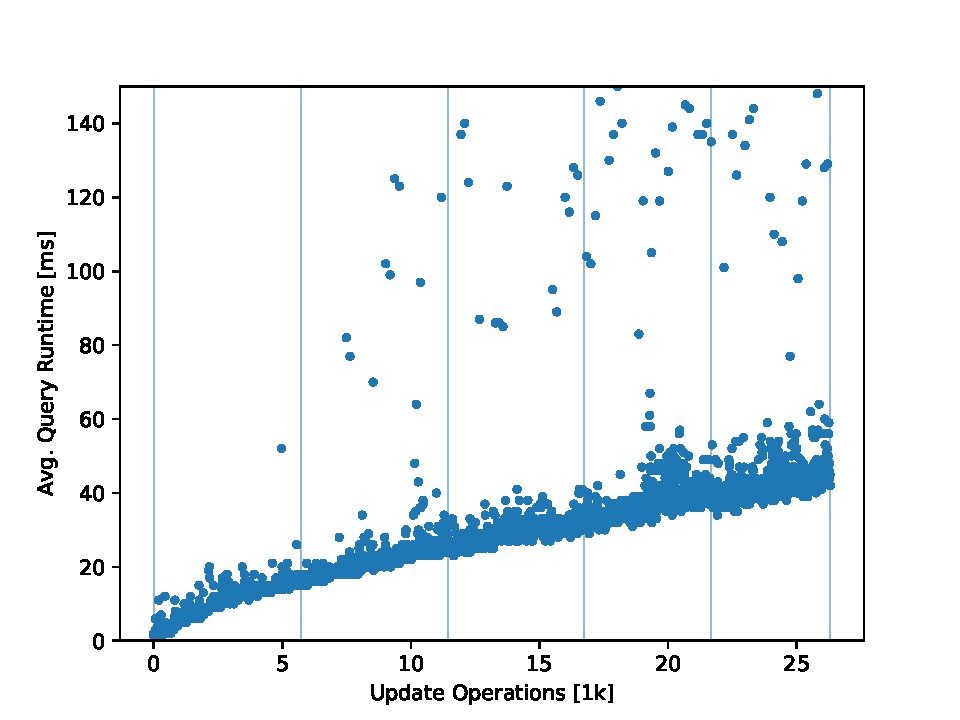
\includegraphics[width=8cm]{query_runtime_synthetic}
    \label{fig:query_runtime_synthetic}
  \end{subfigure}
  \begin{subfigure}{0.49\linewidth}
    \centering
    \caption{Real-World}
    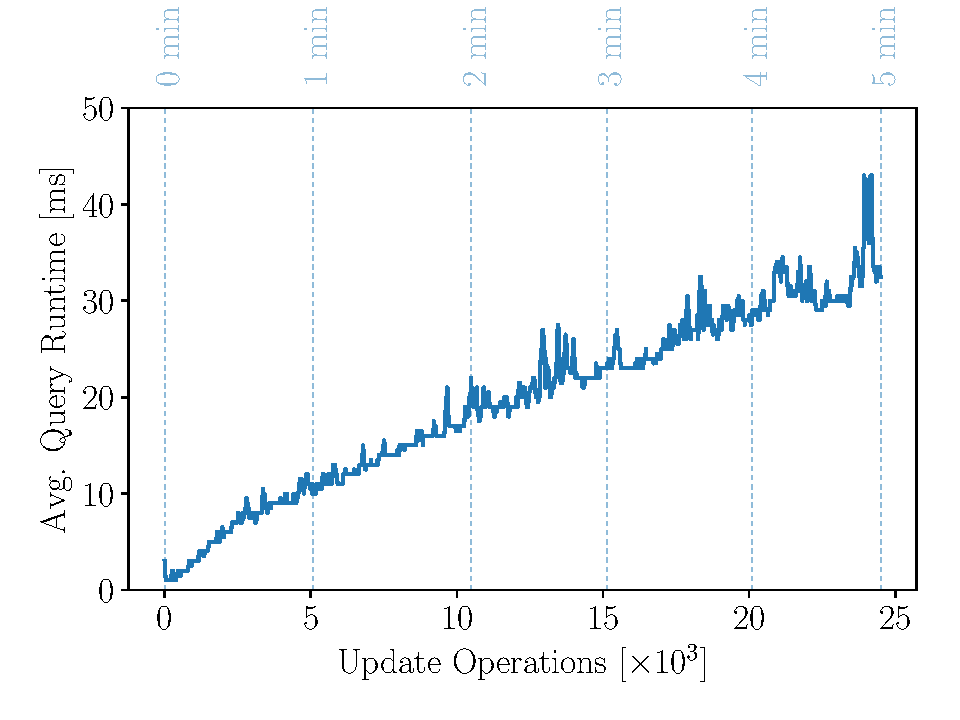
\includegraphics[width=8cm]{query_runtime_real}
    \label{fig:query_runtime_real}
  \end{subfigure}
  \vspace{-0.5cm}
  \caption{Query Runtime over time.}
  \label{fig:query_runtime}
\end{figure}

\subsection{Impact on Query Runtime}

\label{sec:query-runtime}

In this section we study and quantify the impact of unproductive nodes on
query runtime. During query execution, traversing an unproductive node is
useless, because neither the node itself nor any of its descendants are matching
and therefore cannot contribute a query match. We hypothesize that unproductive nodes
significantly slow down queries under a CMS workload.
An index under a CMS workload (see \Cref{sec:application_scenario}) is dominated
by unproductive nodes, that is unproductive nodes constitute a large percentage
of all index nodes.

% We summarize the statements above into the following hypotheses:

% \begin{shaded}
%   \begin{itemize}
%   \item[$H_1$:] WAPI's average query runtime increases over time under a CMS workload.
%   \item[$H_2$:] Unproductive nodes significantly affect WAPI's query runtime
%     under a CMS workload. 
%   \end{itemize}
% \end{shaded}

In order to find supporting evidence for the hypotheses above, we conduct a series of
experiments on Oak. The setup of the  experimental evaluation and
datasets will be described in detail in \Cref{sec:experimental-evaluation}. We
record the query runtime throughout the experiment and present the data below.

\Cref{fig:query_runtime_synthetic,fig:query_runtime_real} show the 
query runtime of the same query as time passes by for the synthetic and
real-world dataset, respectively. 
Each point corresponds to the moving median over 10 time points.
We observe a sublinear increase of the runtime from $2 ms$ to $50 ms$
after running the simulation for $5$ minutes
on the synthetic dataset and an increase from $2 ms$ to $35 ms$ on the
real-world dataset. 
% The identical phenomenon is observed
% in \Cref{fig:trav_nodes_synthetic,fig:trav_nodes_real} respectively because
% query runtime depends on the number of nodes traversed during query execution,
% i.e the increase in query runtime is explained by the increase in total
% traversed nodes per query. 

\begin{figure}[!ht]
  \centering
  \begin{subfigure}{0.49\linewidth}
    \centering
    \caption{Synthetic}
    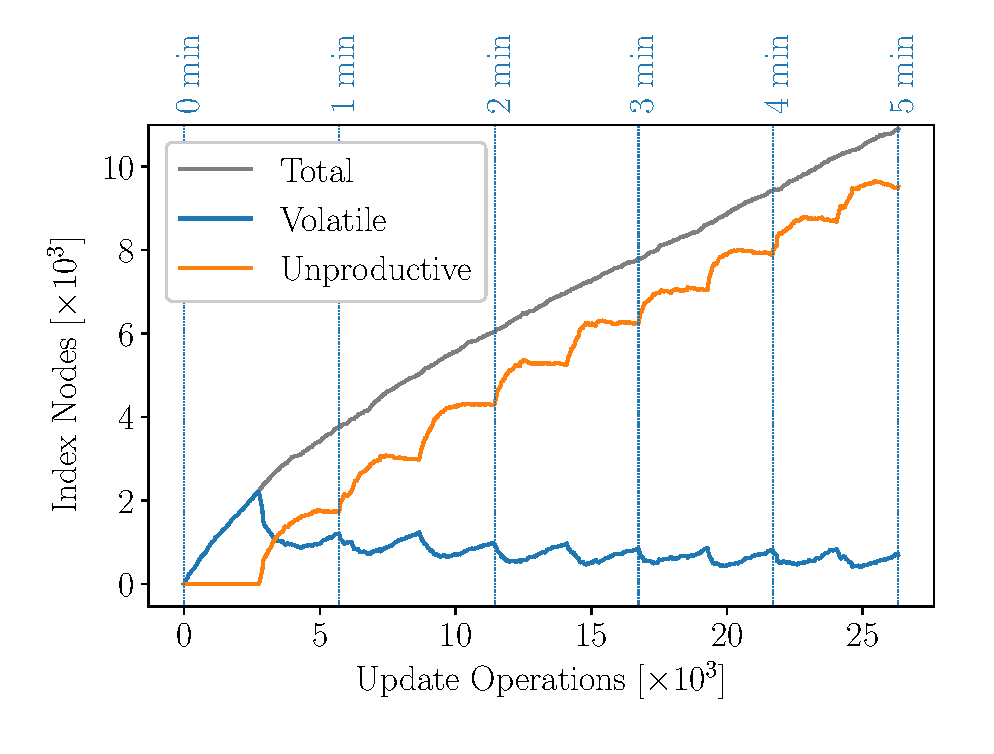
\includegraphics[width=8cm]{trav_nodes_synthetic}
    \label{fig:trav_nodes_synthetic}
  \end{subfigure}
  \begin{subfigure}{0.49\linewidth}
    \centering
    \caption{Real-World}
    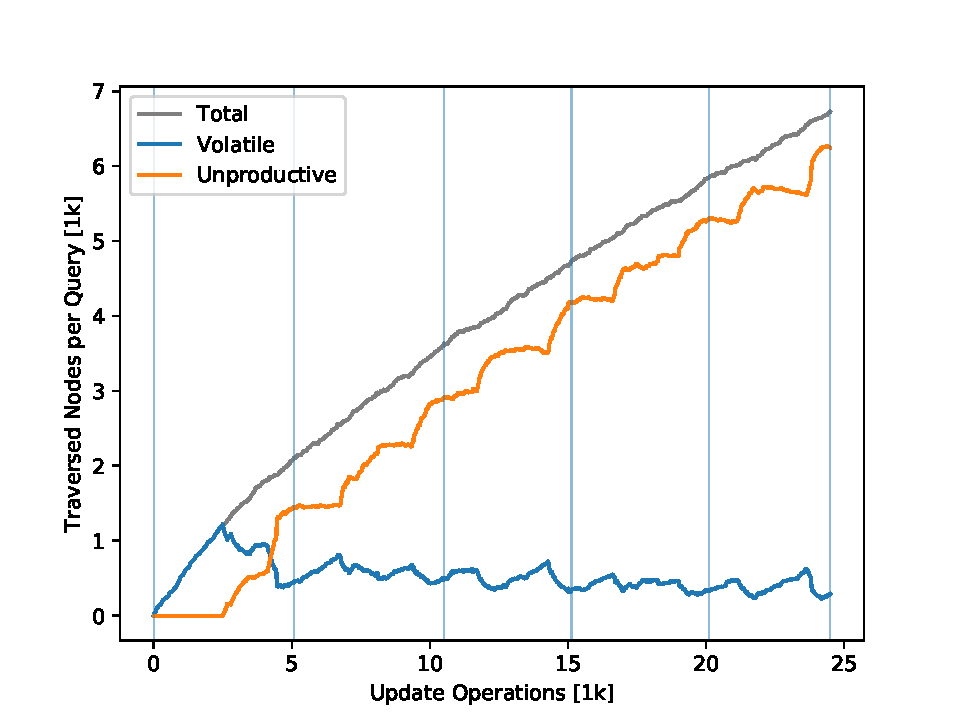
\includegraphics[width=8cm]{trav_nodes_real}
    \label{fig:trav_nodes_real}
  \end{subfigure}
  \vspace{-0.5cm}
  \caption{Index composition during Query Execution.}
  \label{fig:trav_nodes}
\end{figure}

Next, we present data regarding the type of index nodes traversed during query
execution.
\Cref{fig:trav_nodes_synthetic,fig:trav_nodes_real} depict
the total number of traversed nodes in addition to the number of traversed
volatile and unproductive nodes during query execution for each dataset.

The total number of traversed nodes is increasing sublinearly over time. This
explains the increase in query runtime in
\Cref{fig:query_runtime_synthetic,fig:query_runtime_real}.
We believe the index becomes \textit{static} over time.
As time passes, more and more content nodes are randomly
selected by the CMS workload and their corresponding index nodes become
volatile. After some time these nodes, most likely become unproductive and are
not  being pruned from the index anymore.
Therefore, the probability of picking a content node with no corresponding index
node (non-indexed)
decreases over time. Since it becomes less and less likely for a non-indexed content node
to be randomly picked by the CMS workload, the rate of growth of total traversed
index nodes decreases over time. We expect that if we change the workload
sufficiently often, the number of total index nodes converges to the number of
content nodes.

Furthermore, we see the number of volatile nodes have a downward trend from the
30 second mark till the end of the experiment. We believe it becomes less likely
for nodes to become volatile if unproductive nodes are not pruned,
as time passes. When a workload randomly picks a content node whose index node is
unproductive, the index
node becomes matching but was not physically added, thus the volatility count of
the index node
does not increment. In comparison, if the workload randomly picks a non-indexed
content node, the corresponding index node's volatility count increments.
We infer that it is less
likely for an unproductive node to become volatile than a non-indexed one.
Our experimental evaluation suggests that the number of
unproductive nodes increases over time. Therefore it becomes less likely for any
node to become volatile over time. This explains the downward trend of
volatile nodes over time.

The sliding window of length $L$ is set to $30$ seconds, therefore we encounter no
unproductive nodes during the first $30$ seconds of the simulation. Once we
reach the $30$ second mark, the query executor encounters unproductive nodes.
From that point, we observe a steep increase in traversed unproductive nodes.
After $1$ minute, we observe that the total traversed nodes are dominated by
unproductive nodes. The rate of growth of traversed unproductive nodes seems to
decrease over time. When content nodes are picked by the
workload, their corresponding index nodes are inserted into the WAPI, where some
become volatile. When the workload changes, these volatile index nodes most
likely become unproductive and accumulate in the index, hence the number of non-indexed
content nodes decreases. Since less and less non-indexed content nodes are
available to become volatile and thereafter unproductive, the rate of growth of
traversed unproductive nodes decreases.

% More and more content nodes are picked by the workload and
% their corresponding index nodes become volatile. These volatile index nodes most
% likely become unproductive. Therefore it becomes less and less like to pick a
% content node which is non indexed, hence the rate of growth of unproductive
% nodes is decreasing. 

Additionally, we observe the functions of the unproductive and volatile index
nodes having the shape of a cycloid. In \Cref{fig:trav_nodes_synthetic,fig:trav_nodes_real}, each
cusp ($30 s, 60 s, \dots, 300 s$) represents a point in which the workload
changes during the experiment. When the workload changes, we initially see a
steep decrease in volatile nodes. During that phase, more nodes cease to be
volatile than become volatile. Nodes need to reach the threshold in order to
become volatile and few do, since the skew in the workload only picks a subset of
nodes frequently. Before a new workload kicks in, we observe the opposite
phenomenon. More nodes become volatile than cease to be volatile, because many nodes are
on the verge of becoming volatile and therefore need to be picked only a few
times more to become volatile. 

Lastly, we also observe the real-world dataset having a more gentle slope over
the synthetic dataset. Since
the real-world dataset has more content nodes, it is less likely for each
content node to be picked by the workload. Having a smaller chance to be
picked by the workload implies less volatile and consequently less
unproductive nodes in the index.  

\begin{figure}[ht]
  \centering
  \begin{subfigure}{0.49\linewidth}
    \centering
    \caption{Synthetic}
    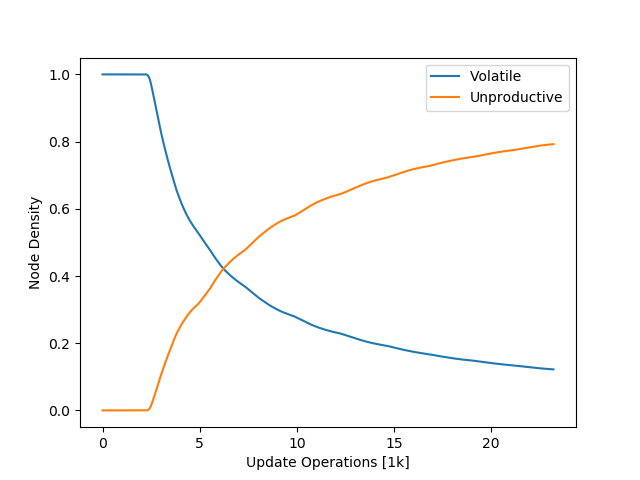
\includegraphics[width=8cm]{trav_node_ratio_synthetic}
    \label{fig:trav_node_ratio_synthetic}
  \end{subfigure}
  \begin{subfigure}{0.49\linewidth}
    \centering
    \caption{Real-World}
    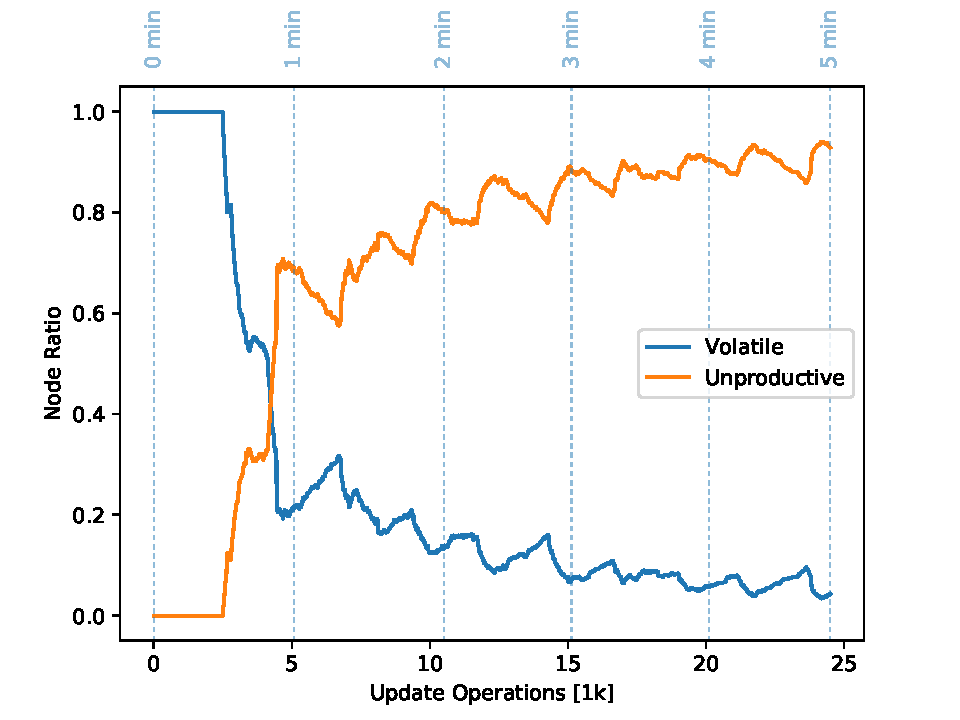
\includegraphics[width=8cm]{trav_node_ratio_real}
    \label{fig:trav_node_ratio_real}
  \end{subfigure}
  \vspace{-0.5cm}
  \caption{Node Ratio during Query Execution.}
  \label{fig:trav_node_ratio}
\end{figure}

\Crefrange{fig:trav_node_ratio_synthetic}{fig:trav_node_ratio_real}
show the ratio of 1) volatile over total and 2) unproductive over total index nodes
over time and update operations from our datasets. These Figures quantify how
strongly unproductive nodes dominate the total traversed nodes. After 5 minutes,
unproductive nodes account for over $80\%$ of the traversed nodes whilst
less than $20\%$ are volatile on the synthetic dataset.
Similarly, on the real-world dataset, we observe $90\%$ traversed unproductive and $10\%$
traversed volatile index nodes.

Concluding, the experiments strongly support our hypothesis. The query runtime
increases by an order of magnitude after 5 minutes. Also, unproductive
nodes, which dominate the index, are accountable for the increase in query runtime. 

\newpage

\section{Cleaning Unproductive Nodes}

In the previous section, we saw how unproductive index nodes slow down query
execution. To prevent unproductive nodes from accumulating in the index, we
need strategies to clean up the index. In the following two subsections, we suggest two
different approaches for dealing with unproductive nodes. We will empirically
investigate their query performance in \Cref{sec:gc-experiment,sec:qtp-experiment}.

\vspace{-0.3cm}

\subsection{Periodic Garbage Collection (GC)}

\label{sec:gc}

First, we propose to clean the index periodically with a garbage collector.
% Using GC, we can guarantee
% that all unproductive nodes are removed from the index. Since GC has to be
% explicitly called, GC takes resources from the system. Executing GC too often
% may decrease system performance.
We add a background process that periodically executes
garbage collection of unproductive nodes wrapped inside 
a single Oak transaction.

The naïve approach for garbage collection is to traverse the entire index subtree,
apply \Cref{def:unproductive-node} to each visited node $n$, and delete $n$ if it
is unproductive. Deciding if $n$ is unproductive, requires us to check that no
descendant $desc(n)$ of $n$ is matching or volatile. Checking the descendants of
each index node $n$ causes naïve GC to have a quadratic time complexity.

\begin{example}[Naïve GC]
  Assume we apply naïve GC to the index subtree depicted in
  \Cref{fig:worst-case}. The subtree resembles the worst-case scenario for GC.
  It contains $n$ nodes, no node is unproductive because the leaf node is matching
  and each internal node has a
  single child. In order to determine if root node $a_1$ is unproductive, we have to
  traverse each
  descendant of $a_1$ and check if it is matching or volatile. The same holds
  for determining if any of $a_1$'s descendants is unproductive. 
  In this example, a node $a_k$ has exactly $n - k$ descendants and to check
  if $a_k$ is unproductive, these $n - k$ descendants need to be traversed.
  %Since $a_1$ has
  %$(n-1)$ descendants, we have to traverse $(n-1)$ nodes to determine if $a_1$
  %is unproductive. For node $a_2$, we have to traverse $(n-2)$ nodes since $a_2$
  %has $(n-2)$ descendants.

  To determine if the $n$ nodes in the subtree rooted at $a_1$ are unproductive,
  we need to traverse the following number of nodes:

  \vspace{-0.5cm}
  
  \begin{align*}
    (n-1) + (n-2) &  + \cdots + (n-n-1) + (n-n) \\
    & = \sum_{k=1}^n n-k \\
    & = \sum_{k=1}^n n - \sum_{k=1}^n k \\
    & = n^2 - \frac{n(n+1)}{2} \\
    & = n^2 - \frac{n^2 + n}{2} \\
    & = \frac{n^2-n}{2} \\
    & = \Theta(n^2)
  \end{align*}
 
  We showed that applying naïve GC on an index subtree of $n$ nodes is bound by
  $\Theta(n^2)$ in the worst case.
 
\end{example}

\begin{figure}
  \centering
  \hspace{2cm}
  \begin{forest}
    [$a_1$,circle,draw,inner sep=7pt
    [$a_2$,circle,draw,inner sep=7pt
    [$\vdots$,base=center,align=center,inner sep=8pt
    [$a_{n-1}$,circle,draw
    [$a_n$,circle,draw,inner sep=7pt] {
      \draw[-] (.east)--++(+1em, -0em)
      node[anchor=west]{pub:now};
    }
    ]
    ]
    ]
    ]
  \end{forest}
  \caption[Worst case scenario during naïve GC]{Worst case scenario during naïve
    Garbage Collection. All internal nodes have a single child. The leaf node
    is matching, therefore no node is unproductive.}
  \label{fig:worst-case}
\end{figure}

By applying a
\textit{postorder tree walk} \cite{Cormen}, we can garbage collect the
index subtree in linear time complexity. The postorder tree walk allows us to
process a node $n$'s descendants before $n$. 
When visiting node $n$ during a postorder tree walk, any unproductive descendant
of $n$ was already pruned, hence no child of $n$ can be unproductive. Thus, if $n$
has at least one child, $n$ cannot be unproductive and therefore checking if $n$
has at least one child, in addition to checking if $n$ is matching or volatile,
is sufficient to determine if $n$ is unproductive, when applying a postorder
tree walk.
% Checking if $n$ has children is sufficient
% to determine if $n$ has matching or volatile descendants. Any child of $n$
% is guaranteed to be productive and by having a productive child, $n$ is also
% productive. 
\Cref{fig:postorder} depicts a postorder tree walk on snapshot $G^3$ from
\Cref{fig:unproductive_nodes}. The numbers represent the
order in which the nodes are checked and pruned if unproductive. A node's
descendants are always evaluated before the node itself.

\begin{figure}[h]
  \centering
  \small
  \begin{forest}
    [
    [$\lambda$:$i$, name=i
    [$\lambda$:pub, name=i_pub
    [$\lambda$:now, name=i_pub_now
    [$\lambda$:$a$, name=i_pub_now_a
    [$\lambda$:$b$, name=i_pub_now_a_b
    [$\lambda$:$d$, name=i_pub_now_a_b_d] {
      \draw[-,gray] (.south west)--++(-5em, -1em)
      node[anchor=east]{1};
    }
    ] {
      \draw[-,gray] (.south west)--++(-5em, -1em)
      node[anchor=east]{2};
    }
    [,phantom]
    [,phantom]
    [$\lambda$:$c$, name=i_pub_now_a_c
    [$\lambda$:$e$ \\ pub:now, align=center, base=bottom, name=i_pub_now_a_c_e] {
      \draw[-,gray] (.south east)--++(5em, -1em)
      node[anchor=west]{3};
    }
    ] {
      \draw[-,gray] (.south east)--++(5em, -1em)
      node[anchor=west]{4};
    }
    ] {
      \draw[-,gray] (.south west)--++(-5em, -1em)
      node[anchor=east]{5};
    }
    ] {
      \draw[-,gray] (.south west)--++(-5em, -1em)
      node[anchor=east]{6};
    }
    ] {
      \draw[-,gray] (.south west)--++(-5em, -1em)
      node[anchor=east]{7};
    }
    ] 
    [$\lambda$:$a$
    [$\lambda$:$b$
    [$\lambda$:$d$]
    ]
    [$\lambda$:$c$
    [$\lambda$:$e$ \\ pub:now, align=center, base=bottom]
    ]
    ]
    ]
    \draw[-,dotted] (i_pub) to[out=west, in=west] (i_pub_now);
    \draw[-,dotted] (i_pub_now) to[out=west, in=west] (i_pub_now_a);
    \draw[-,dotted] (i_pub_now_a) to[out=west, in=west] (i_pub_now_a_b);
    \draw[->,dotted] (i_pub_now_a_b) to[out=west, in=west] (i_pub_now_a_b_d);
    \draw[->,dotted] (i_pub_now_a_b_d) to[out=east, in=south east] (i_pub_now_a_b);
    \draw[-,dotted] (i_pub_now_a_b) to[out=east, in=west] (i_pub_now_a_c);
    \draw[->,dotted] (i_pub_now_a_c) to[out=west, in=west] (i_pub_now_a_c_e);
    \draw[->,dotted] (i_pub_now_a_c_e) to[out=east, in=east] (i_pub_now_a_c);
    \draw[->,dotted] (i_pub_now_a_c) to[out=north, in=south east] (i_pub_now_a);
    \draw[->,dotted] (i_pub_now_a) to[out=east, in=south east] (i_pub_now);
    \draw[->,dotted] (i_pub_now) to[out=east, in=south east] (i_pub);
  \end{forest}
  \caption[Postorder tree walk]{Postorder tree walk on the index subtree rooted at
    \texttt{/i} of $G^3$. The numbers represent the order the corresponding nodes where
    visited, e.g. \texttt{/i/pub/now/a/b/d} was visited first,
    \texttt{/i/pub/now/a/b} second, etc.}
  \label{fig:postorder}
\end{figure}


\Cref{algo:periodic_gc_wapi} prunes all
unproductive descendants of the index subtree rooted at \texttt{/i}. The algorithm traverses
the subtree rooted at \texttt{/i} using a postorder tree walk. If a descendant $n \in
desc(\texttt{/i})$ has no children and is neither matching, nor
volatile, it is unproductive and therefore pruned from the index. If $n$ has at least
one child, we infer
that $n$ has at least one matching or volatile descendant, thus $n$ cannot be
unproductive. The postorder tree walk ensures
that the algorithm prunes a child before its parent node. This guarantees that
all unproductive nodes are pruned.

\begin{algorithm}
  \caption{GarbageCollect}
  \DontPrintSemicolon
  \For{node $n \in desc(\texttt{/i})$ in postorder tree walk}{
    \If{$chd(n) = \emptyset \land \neg matching(n) \land \neg volatile(n)$}{
      delete node $n$\;
    }
  }
  \label{algo:periodic_gc_wapi}
\end{algorithm}

\vspace{-1cm}

\begin{figure}[H]
  \centering
  \begin{large}
    $$ G^3 \xrightarrow{\quad T_4 \quad} G^4$$
  \end{large}
\begin{subfigure}{0.30\textwidth}
  \centering
  \scriptsize
  \begin{framed}
    \begin{forest}
      [
      [$\lambda$:$i$
      [$\lambda$:pub
      [$\lambda$:now
      [$\lambda$:$a$
      [$\lambda$:$b$, color=Orange
      [$\lambda$:$d$, color=Orange]
      ]
      [$\lambda$:$c$, color=RoyalBlue
      [$\lambda$:$e$ \\ pub:now, color=RoyalBlue, align=center, base=bottom]
      ]
      ]
      ]
      ]
      ]
      [,phantom]
      [$\lambda$:$a$
      [$\lambda$:$b$
      [$\lambda$:$d$]
      ]
      [$\lambda$:$c$
      [$\lambda$:$e$ \\ pub:now, align=center, base=bottom]
      ]
      ]
      ]
    \end{forest}
  \end{framed}
  \footnotesize{
    Snapshot $G^3$

    $t(G^3) = t + 3$
  }
\end{subfigure}
\begin{subfigure}{0.30\textwidth}
  \centering
  \scriptsize
  \begin{framed} 
    \begin{forest}
      [
      [$\lambda$:$i$
      [$\lambda$:pub
      [$\lambda$:now
      [$\lambda$:$a$
      [,phantom]
      [,phantom]
      [$\lambda$:$c$, color=RoyalBlue
      [$\lambda$:$e$ \\ pub:now, color=RoyalBlue, align=center, base=bottom]
      ]
      ]
      ]
      ]
      ]
      [$\lambda$:$a$
      [$\lambda$:$b$
      [$\lambda$:$d$]
      ]
      [$\lambda$:$c$
      [$\lambda$:$e$ \\ pub:now, align=center, base=bottom]
      ]
      ]
      ]
    \end{forest}
  \end{framed}
  \footnotesize{
    Snapshot $G^4$

    $t(G^4) = t + 4$
  }
\end{subfigure}
\caption[GC applied on Oak]{Garbage collection applied on Oak.
  Assume nodes \texttt{/i/pub/now/a/b/d} and \texttt{i/pub/now/a/b} are
  unproductive (color-coded orange) in snapshot $G^3$. Garbage collection is
  executed during transaction $T_4$. $G^4$ is the committed snapshot.}
\label{fig:periodic_gc}
\end{figure}

\begin{example}[Periodic GC]
  \Cref{fig:periodic_gc} shows snapshot $G^3$ from
  \Cref{fig:unproductive_nodes}. Index nodes \texttt{/i/pub/now/a/b/d}
  and \texttt{/i/pub/now/a/b} are unproductive in snapshot $G^3$, as explained
  in \Cref{ex:unproductive-node}. Oak's background process executes garbage
  collection during $T_4$. While executing GC, the index subtree of $G^3$ is
  traversed in postorder.
  The first unproductive node we visit and prune is
  \texttt{/i/pub/now/a/b/d}. Next, the garbage collector visits and prunes
  \texttt{/i/pub/now/a/b}. No further unproductive node is left for pruning. We
  see the cleaned index after garbage collection in snapshot $G^4$.
\end{example}

\begin{figure}[H]
  \small
  \begin{framed}
\begin{minted}{java}
/**
 * Removes any unproductive descendant from the index subtree.
 *
 * @param root: latest Oak snapshot 
 */
void garbageCollect(Root root) {

    /* index subtree root */
    Tree indexRoot = root.getTree(OAK_INDEX_PATH);

    /* filter nodes which have children, are matching or volatile */
    for (Tree unproductiveNode : filter(
            (Tree n) -> n.getChildrenCount(1) == 0 &&
                        !isMatching(n) &&
                        !isVolatile(n),

            /* postorder tree walk iterable */
            postOrder(indexRoot)
    ) {
        unproductiveNode.remove();
    }
}
\end{minted}
  \end{framed}
  \caption[Periodic GC implemented in Java]{Periodic Garbage Collection
    implemented in Java.}
  \label{fig:java_periodic_gc}
\end{figure}

\Cref{fig:java_periodic_gc} shows the implementation of the periodic
GC in Java inside Apache Jackrabbit Oak. Calling \texttt{postOrder()} returns a
lazy sequence of nodes
which correspond to a postorder tree walk of the index subtree (cf.
\Cref{fig:java_postorder} in the Appendix). Next, using \texttt{filter()} we
remove any node
that has children, is matching or volatile from the sequence. All other nodes are
unproductive and therefore pruned from the index.

By applying periodic GC on Oak, we introduce a new
parameter. \textit{GC Period $T$} defines how often garbage collection is run by
the background process on Oak. If we pick a smaller
period $T$, garbage collection is run more often and this
reduces the number of unproductive nodes in the index. As a result, we
increase the query performance of Oak,
since the query executor has to traverse less unproductive nodes on average.

It is also worth mentioning that GC uses system resources in order to clean the
index. If run too often, GC might degrade query performance, because the system
is busy cleaning the index, instead of processing queries.

We suggest running GC when the system is not busy executing queries, e.g, every
day during the 
early morning hours. Like so, garbage collection minimally interferes with other
transactions. We will revisit GC period in \Cref{sec:periodicity}, where we
conduct an experiment in order to determine the impact of period $T$ on
unproductive nodes. 

\subsection{Query-Time Pruning (QTP)}

While periodic garbage collection is explicitly executed by Oak in order to
clean unproductive nodes, Query-Time Pruning is an approach which cleans
unproductive nodes whilst Oak answers queries. Doing so, we benefit by
avoiding the cost of explicitly traversing the index in comparison to GC.  

Frequent queries also benefit from QTP. If a query is executed for the first
time, QTP cleans all unproductive nodes traversed during query execution.
If the query is executed a second time shortly thereafter and  no new nodes
become unproductive in the meantime, the query executor encounters no
unproductive nodes anymore and therefore the query is answered faster.

If the path filter \texttt{m} of CAS query $Q(\texttt{k},\texttt{v},\texttt{m})$
(cf. \Cref{def:cas-query}) changes often, 
the query executor starts traversing new subtrees in the index
and consequently, some subtrees are not queried anymore. If an unproductive
node is a member of a subtree that is not queried anymore, it is not pruned and
remains in the index.
Such unproductive nodes waste space because they contain no data but do not
impact query performance since they are not traversed during query execution.

% The drawback of QTP are \textit{leftover}
% unproductive nodes we get from subtrees which are not queried anymore. Leftover
% unproductive nodes waste space but do not impact query performance since they are
% not traversed during query execution.

When using QTP to query for all descendants of a content node with path \texttt{m},
we apply a postorder tree walk.
With the postorder tree walk, we traverse and clean all unproductive nodes in
the subtree of $\texttt{/i/k/v/m} =
\texttt{/i/k/v/} \lambda_1 \texttt{/} \dots \texttt{/} \lambda_d$ in linear time
complexity, as explained in \Cref{sec:gc}. In the same Section, we mention that
during a postorder tree walk,
checking if node $n$ has at least one child, in addition to checking if $n$ is
matching or volatile, is sufficient to determine if $n$ is unproductive.
% If any descendant $n \in
% desc(\texttt{/i/k/v/m})$ has at least one child, we
% infer that it has at least one matching or volatile descendant, therefore making
% $n$ productive.
The postorder tree walk ensures that the algorithm prunes
a child before its parent node. This guarantees that all unproductive nodes are
pruned in the subtree rooted at \texttt{/i/k/v/m}.

\Cref{algo:query_qtp_wapi} takes a CAS query
$Q(\texttt{k},\texttt{v},\texttt{m})$ as an argument, where
\texttt{k} is a property, \texttt{v} a value and \texttt{m} a content node's
path. We initialize set $r$
as the empty set. $r$ will hold all content nodes satisfying the CAS query (cf.
\Cref{def:cas-query}).
We traverse any descendant $n$ of $\texttt{/i/k/v/m} =
\texttt{/i/k/v/}\lambda_1\texttt{/}\dots\texttt{/}\lambda_d$ in a postorder tree
walk. If node $n$ is matching, we add its corresponding content node to
$r$ and proceed to the next descendant. If node $n$ has no children and is
neither matching, nor volatile, it is unproductive and therefore pruned from the index.
After we finish traversing all descendants $n$, we return the result set $r$.

\begin{algorithm}
  \caption{QueryQTP}
  \DontPrintSemicolon
  \KwData{Query $Q(k, v, m)$, where $k$ is a property, $v$ a value and $m$ (=
    $\texttt{/}\lambda_1\texttt{/}\dots\texttt{/}\lambda_d$) a
    content node's path.}
  \KwResult{A set of nodes satisfying $Q(k,v,m)$}
  $r \longleftarrow \emptyset$\;
  \For{node $n \in
    desc(\texttt{/i/k/v/}\lambda_1\texttt{/}\dots\texttt{/}\lambda_d)$ in postorder tree walk}{
    \uIf{$matching(n)$}{
      $r \longleftarrow r \cup \{ *n \}$\;
    }
    \ElseIf{$chd(n) = \emptyset \land \neg volatile(n)$}{
      delete node $n$
    }
  }
  \Return{r}\;
  \label{algo:query_qtp_wapi}
\end{algorithm}


\begin{figure}[H]
  \vspace{-0.5cm}
  \centering
  \begin{large}
    $$ G^5 \xrightarrow{\quad T_6 \quad} G^6$$
  \end{large}
\begin{subfigure}{0.40\textwidth}
  \centering \scriptsize{
    \begin{framed}
      \begin{forest}
        [
        [$\lambda$:$i$
        [$\lambda$:pub
        [$\lambda$:now
        [$\lambda$:$a$
        [$\lambda$:$b$
        [$\lambda$:$d$ \\ pub:now, align=center, base=bottom]
        [$\lambda$:$e$ \\ \vspace{-1mm}, color=Orange, align=center, base=bottom]
        ]
        [$\lambda$:$c$, color=Orange
        [,phantom]
        ]
        ]
        ]
        ]
        ]
        [$\lambda$:$a$
        [$\lambda$:$b$
        [$\lambda$:$d$ \\ pub:now, align=center, base=bottom]
        [$\lambda$:$e$ \\ \vspace{-1mm}, align=center, base=bottom]
        ]
        [$\lambda$:$c$
        [,phantom]
        ]
        ]
        ]
      \end{forest}
    \end{framed}
  } \footnotesize{ Snapshot $G^5$ }
\end{subfigure}
\begin{subfigure}{0.40\textwidth}
  \centering \scriptsize{
    \begin{framed}
      \begin{forest}
        [
        [$\lambda$:$i$
        [$\lambda$:pub
        [$\lambda$:now
        [$\lambda$:$a$
        [$\lambda$:$b$
        [$\lambda$:$d$ \\ pub:now, align=center, base=bottom]
        [,phantom]
        ]
        [$\lambda$:$c$, color=Orange
        [,phantom]
        ]
        ]
        ]
        ]
        ]
        [$\lambda$:$a$
        [$\lambda$:$b$
        [$\lambda$:$d$ \\ pub:now, align=center, base=bottom]
        [$\lambda$:$e$ \\ \vspace{-1mm}, align=center, base=bottom]
        ]
        [$\lambda$:$c$
        [,phantom]
        ]
        ]
        ]
      \end{forest}
    \end{framed}
  } \footnotesize{ Snapshot $G^6$ }
\end{subfigure}
\caption[QTP applied on Oak]{Query-Time Pruning applied on Oak. Assume nodes
  \texttt{/i/pub/now/a/b/e} and \texttt{/i/pub/now/a/c} are
  unproductive in snapshot $G^5$. Transaction $T_6$ executes CAS query
  $Q(\texttt{pub},\texttt{now},\texttt{/a/b})$ which queries for all descendants
  of \texttt{/a/b} with ``pub'' set to ``now'' and commits the resulting
  snapshot $G^6$. QTP is used during query execution.}
  \label{fig:qtp}
\end{figure}

\begin{example}[QTP]
  Consider \Cref{fig:qtp}. Transaction $T_6$ executes CAS query
  $Q(\texttt{pub},\texttt{now},\texttt{/a/b})$ which queries for all descendants
  of \texttt{/a/b} with ``pub'' set to ``now'' in snapshot $G^5$. Assume the
  query executor uses QTP and nodes \texttt{/i/pub/now/a/b/e} and
  \texttt{/i/pub/now/a/c} are unproductive. The
  query executor traverses all descendants of \texttt{/i/pub/now/a/b} and
  therefore prunes the unproductive index node \texttt{/i/pub/now/a/b/e}. Since
  the other unproductive index node (\texttt{/i/pub/now/a/c}) is not traversed
  during query execution,
  it is not pruned and remains in the index unproductive. The resulting
  snapshot $G^6$ is committed by $T_6$ after finishing query execution.
\end{example}

\Cref{fig:java_qtp} shows the Java implementation of QTP in Oak. The algorithm
takes a property \texttt{k}, value \texttt{v}, path \texttt{m}, a
\texttt{Root} and returns a lazy sequence of content nodes satisfying
the CAS query $Q(\texttt{k},\texttt{v},\texttt{m})$. By Calling
\texttt{postOrder()} we get a sequence of nodes representing a
postorder tree walk in the subtree rooted at \texttt{/i/k/v/m}. We remove any
node that is not
matching from the sequence using \texttt{filter()}. If a node has no children
and is neither matching,
nor volatile, it is unproductive and we prune it from the index.

\vspace{1cm}

\begin{figure}[H]
  \scriptsize
  \begin{framed}    
\begin{minted}{java}
/**
 * Answers a CAS Query and prunes traversed unproductive index nodes.
 *
 * @param k: Property we query for
 * @param v: Value we query for
 * @param m: Path of content node which the descendants we query for
 * @param root: Latest Oak snapshot
 * @returns An iterable with content nodes satisfying the CAS query
 */
Iterable<Tree> QueryQTP(String k, String v, String m, Root root) {

    /* e.g.: /oak:index/pub/:index/now */
    String indexRootPath = concat(OAK_INDEX_PATH, k, v); 

    /* e.g.: /oak:index/pub/:index/now/a */
    String queryNodePath = concat(indexRootPath, m);

    /* map index nodes to corresponding content nodes */
    return map((Tree n) -> {
            return root.getTree(relativize(indexRootPath, n.getPath()));
        },

        /* filter non-matching index nodes */
        filter((Tree n) -> {
                
                boolean isMatchingMemo = isMatching(n);

                /* prune if no children, not matching and not volatile */
                if (n.getChildrenCount(1) == 0 &&
                    !isMatchingMemo &&
                    !isVolatile(n)
                ) {
                    n.remove();
                }
                return isMatchingMemo;
            },

            /* postorder tree walk of descendants of /i/k/v/m */
            postOrder(root.getTree(queryNodePath))
        )
    );
}
\end{minted}
  \end{framed}
  \caption[QTP implemented in Java]{Query-Time Pruning implemented in Java.}
  \label{fig:java_qtp}
\end{figure}

\newpage\null\thispagestyle{empty}\newpage

\section{Experimental Evaluation}

\label{sec:experimental-evaluation}

\subsection{Goals}

The goal of our experimental evaluation is to compare GC and QTP under
different parameterizations and workloads.
In \Cref{sec:threshold,sec:sliding-window,sec:skew,sec:update-query-ratio} we
see how the parameters volatility threshold $\tau$, sliding window length $L$,
workload skew $s$ and update to query ratio, impact unproductive nodes in the
index subtree.
These parameters directly impact the number of volatile nodes and therefore can affect
the production of unproductive nodes in the index.
In \Cref{sec:gc-experiment}, we evaluate the query performance of GC and in
\Cref{sec:periodicity} we investigate how GC period $T$ affects GC's performance.
The experimental methodolody used on GC is also applied on QTP in \Cref{sec:qtp-experiment}.
Lastly, \Cref{sec:comparison} compares GC and QTP directly and suggests under which
circumstances one might use periodic GC over QTP, and vice versa.
%side and list their differences in \Cref{sec:gc-qtp-performance}. Next, we
%investigate effects GC period has on garbage collection in \Cref{sec:periodicity}.
%Executing GC more often might increase system
%performance since more unproductive nodes are pruned. Also, we conduct an
%experiment in \Cref{sec:skew} in order to examine how
%workload skew impacts the performance of GC and QTP. Finally, we run simulations
%in order to see how the update to query ratio affects the performance of GC and
%QTP in \Cref{sec:update-query-ratio}.


\subsection{Preliminaries}

\subsubsection{Setup}

We use a volatility threshold $\tau = 5$ and sliding window of length $L = 30s$ as defaults,
unless otherwise noted.
All experiments are conducted on a 15'' Macbook Pro 2015 inside
a virtual machine running Linux Arch.\footnote{https://www.archlinux.org/about/}
We allocate 4 out of 8 virtual cores (Intel i7-4980HQ 2.7 - 4.0 GHz) to the virtual
machine and 12 GB of RAM. We allocated half the available virtual cores of the machine
because we wanted to ensure the machine's limited CPU cooling performance will not affect the simulations.

\subsubsection{Datasets}

\label{sec:datasets}

\begin{figure}[h]
  \centering
  \begin{subfigure}{0.49\linewidth}
    \centering
    \caption{Synthetic}
    \tiny
    \begin{forest}
      [,circle,draw
      [,circle,draw
      [,circle,draw
      [,circle,draw
      [,circle,draw]
      [,circle,draw] 
      ]
      [,circle,draw
      [,circle,draw]
      [,circle,draw]
      ]
      ]    
      [,circle,draw
      [,circle,draw
      [,circle,draw]
      [,circle,draw] 
      ]
      [,circle,draw
      [,circle,draw]
      [,circle,draw]
      ]
      ] 
      ]
      [,circle,draw
      [,circle,draw
      [,circle,draw
      [,circle,draw]
      [,circle,draw] 
      ]
      [,circle,draw
      [,circle,draw]
      [,circle,draw]
      ]
      ]
      [,circle,draw
      [,circle,draw
      [,circle,draw]
      [,circle,draw] 
      ]
      [,circle,draw
      [,circle,draw]
      [,circle,draw]
      ]
      ]  
      ]
      ]
    \end{forest}
\end{subfigure}
\begin{subfigure}{0.49\linewidth}
  \centering
  \caption{Real-World}
    \tiny
    \begin{forest}
      [,circle,draw
      [,phantom]
      [,circle,draw
      [,circle,draw
      [,circle,draw]
      [,circle,draw
      [,circle,draw]
      ]
      [,circle,draw]
      [,circle,draw]
      [,circle,draw
      [,circle,draw]
      ]
      ]
      ]
      [,phantom]
      [,phantom]
      [,phantom]
      [,circle,draw]
      [,circle,draw
      [,circle,draw
      [,circle,draw
      [,circle,draw]
      [,circle,draw]
      [,circle,draw]
      [,circle,draw]
      [,circle,draw]
      [,circle,draw]
      [,circle,draw]
      ]
      [,circle,draw
      [,circle,draw]
      ]
      ]
      ]
      ]
    \end{forest}
  \end{subfigure}
  \caption{Excerpts of both datasets visualized.}
  \label{fig:dataset}
\end{figure}


We use two datasets in our experiments. Each dataset resembles the content
subtree of an Oak instance. The \textit{synthetic} dataset is a complete binary
tree of height 19, that is a binary tree in which all leaf nodes have depth 19
\cite{Cormen}. It contains $2^{20} \approx 10^6$ nodes, of which 50\% are leaf
nodes. Each node has a mean depth and fanout of 18 and 2, respectively. The
\textit{real-world} dataset is based on DELL's website (http://dell.com)
which is built on top of Adobe's AEM that uses Oak.\footnote{https://wwwimages2.adobe.com/content/dam/acom/en/customer-success/pdfs/dell-case-study.pdf}
It is sparser than the synthetic dataset and contains $13 \cdot 10^6$
nodes, 65\% of which are leaf nodes. Each node has a mean depth and fanout of
$13.68$ and exactly 1, respectively. The tree's nodes have a max depth and fanout of 24
and 1729, respectively. Since the dataset is so sparse, there exist many nodes with a single child and few with many children, forming linked lists \cite{Cormen} of nodes
sometimes. \Cref{fig:dataset} shows a sample subtree for each dataset.

\subsubsection{Workload}

\label{sec:workload}

In \Cref{sec:application_scenario}, we introduced the characteristics of a CMS
workload. Using a running example we explained that a CMS workload is skewed,
update-heavy, changing and CMSs frequently make use of a job-queuing system.
For our experiments, we designed a workload that has the noted characteristics.

The workload randomly draws content nodes and executes an update on them.
The workload is only allowed to draw content nodes with depth greater than
the mean depth. Drawing nodes with a depth greater than average makes query
execution more expensive because Oak has to traverse more nodes when answering
queries, on average. We denote the set of nodes of the content subtree with
depth greater than the mean depth as the \textit{lower content subtree}.

In order to have skew, we incorporate the Zipf distribution. The Zipf
distribution picks a small subset of nodes more frequent than others. 
Let $N$ be the number of nodes inside the lower content subtree.
We randomly and uniquely assign an integer $k \in [1, N]$ to each node in the
lower content subtree, creating 
a $k \rightarrow$ node mapping. The probability of randomly drawing the $k$-th node 
from the lower content subtree according to the Zipf distribution is:

\begin{large}

    $$ Zipf(k,N,s) = \bigg(k^s \cdot \sum_{i=1}^{N}\frac{1}{i^s} \bigg)^{-1} $$

\end{large}

The $k$-th node corresponds to the node which is assigned integer $k$ in the mapping.
Skewness $s$ of the Zipf distribution is parameterizable and we use $s=1$ by
default in our experiments, unless otherwise noted. By having a smaller skew,
the subset of nodes which is frequently selected, becomes bigger.
With $s=0$, the Zipf distribution corresponds to the uniform distribution
and every node has equal probability to be drawn.
In \Cref{sec:skew}, we make an experiment to determine skew's impact on
unproductive nodes.

\begin{figure}[h]
  \centering
   \begin{subfigure}{0.49\linewidth}
    \centering
    \caption{Synthetic}
    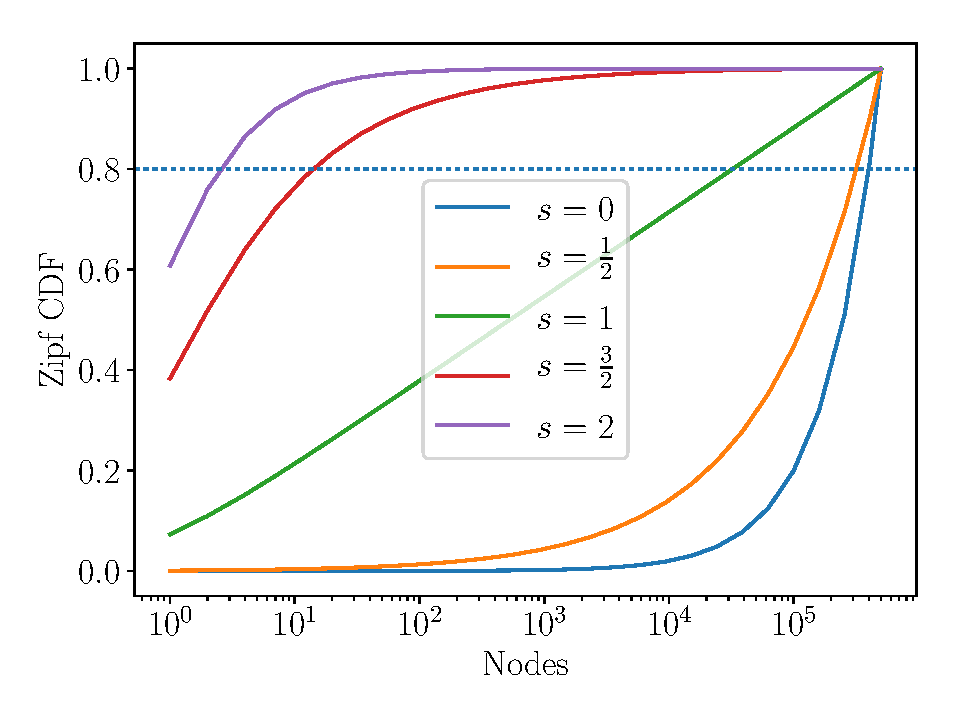
\includegraphics[width=8cm]{cdf_synthetic}
    \label{fig:cdf_synthetic}
  \end{subfigure}
  \begin{subfigure}{0.49\linewidth}
    \centering
    \caption{Real-World}
    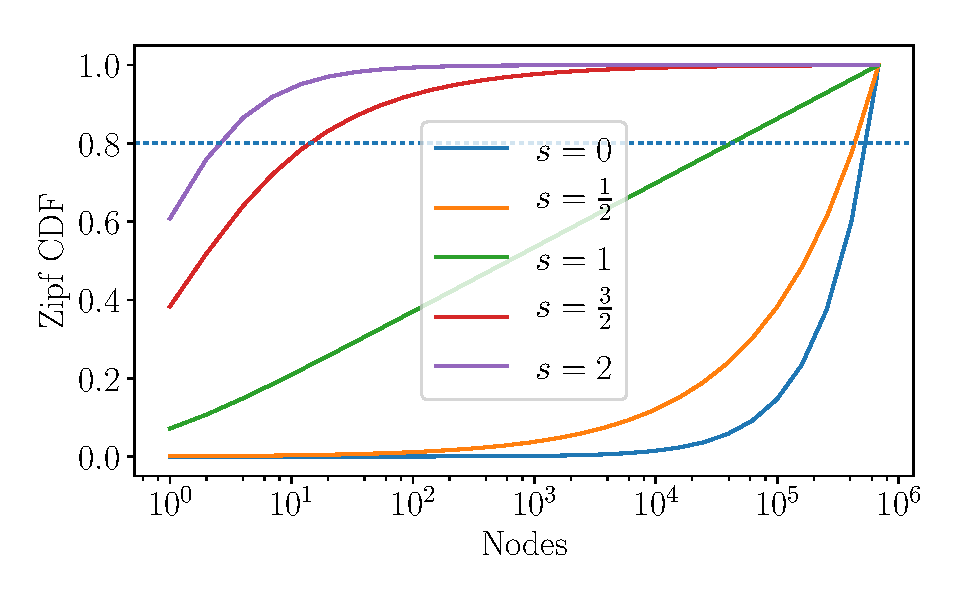
\includegraphics[width=8cm]{cdf_real}
    \label{fig:cdf_real}
  \end{subfigure}
  \vspace{-0.5cm}
  \caption{CDF for the Zipf distribution for both datasets.}
\end{figure}

\Cref{fig:cdf_synthetic,fig:cdf_real} show Zipf's Cumulative Distribution
Function (CDF) for both datasets and skew values $s \in \{0, \frac{1}{2}, 1, \frac{3}{2}, 2\}$.
If we randomly draw a large sample of nodes according to the distribution with $s=1$,
80\% of these nodes are amongst the same 30k nodes (6\% of all nodes) on the synthetic
dataset and 40k nodes (5.9\% of all nodes) on the real-world dataset.

A CMS workload is also update-heavy. To simulate this, we execute many update 
operations before
executing a query operation. We fix the default update to query ratio to 10:1, i.e., 
that is 10 update operations are executed for each query operation. In
\Cref{sec:update-query-ratio}, we evaluate and compare GC and QTP under various
update to query ratios.

Additionally, the workload we design has to be changing. We periodically permute 
the node mappings by reassigning a new random and unique integer $k \in [1,N]$ to each
node from the dataset in order to change the hotspots of the simulation, that is
the subset of nodes which are frequently updated.
We change the hotspot by default every 30 seconds. During a 5 minute
experiment we expect 10 different workloads.

Lastly, the workload has to simulate a job-queuing system. An update operation
executed during the experiment is composed from two actions. We first set the
``pub'' = ``now'' property-value pair to the node and then consecutively remove
it. The actions simulate a node being inserted into the queue and then being
processed and removed. Using our designed update operation, there can be at most
one matching index node at any instance of time.

\begin{figure}[h]
  \centering
  \begin{subfigure}{0.20\textwidth}
    \centering
    \scriptsize
    \begin{forest}
      [,circle,draw,fill=Yellow
      [,circle,draw,fill=Yellow
      [,circle,draw,fill=Orange
      ]
      [,circle,draw,fill=Yellow
      [,circle,draw,fill=Red]
      [,phantom]
      ]
      ]
      [,circle,draw,fill=Yellow
      [,phantom]
      [,circle,draw,fill=Yellow
      [,circle,draw,fill=Yellow
      [,circle,draw,fill=Yellow]
      [,circle,draw,fill=Yellow]
      ]
      [,circle,draw,fill=Orange]
      ]
      ]
      ]
    \end{forest}
  \end{subfigure}
  \begin{subfigure}{0.10\textwidth}
    \centering
    $\longrightarrow$
  \end{subfigure}
  \begin{subfigure}{0.20\textwidth}
    \centering
    \scriptsize
    \begin{forest}
      [,circle,draw,fill=Yellow
      [,circle,draw,fill=Yellow
      [,circle,draw,fill=Yellow
      ]
      [,circle,draw,fill=Yellow
      [,circle,draw,fill=Yellow]
      [,phantom]
      ]
      ]
      [,circle,draw,fill=Orange
      [,phantom]
      [,circle,draw,fill=Yellow
      [,circle,draw,fill=Yellow
      [,circle,draw,fill=Orange]
      [,circle,draw,fill=Red]
      ]
      [,circle,draw,fill=Orange]
      ]
      ]
      ]
    \end{forest}
  \end{subfigure}
  \begin{subfigure}{0.10\textwidth}
    \centering
    $\longrightarrow$
  \end{subfigure}
  \begin{subfigure}{0.20\textwidth}
    \centering
    \scriptsize
    \begin{forest}
      [,circle,draw,fill=Yellow
      [,circle,draw,fill=Yellow
      [,circle,draw,fill=Orange
      ]
      [,circle,draw,fill=Yellow
      [,circle,draw,fill=Yellow]
      [,phantom]
      ]
      ]
      [,circle,draw,fill=Yellow
      [,phantom]
      [,circle,draw,fill=Yellow
      [,circle,draw,fill=Red
      [,circle,draw,fill=Orange]
      [,circle,draw,fill=Yellow]
      ]
      [,circle,draw,fill=Yellow]
      ]
      ]
      ]
    \end{forest}
  \end{subfigure}

  \caption[CMS Workloads visualized]{CMS Workloads visualized.
  Red shaded nodes are the most frequently selected nodes.}
  \label{fig:workload}
\end{figure}

\Cref{fig:workload} depicts heatmaps of a content subtree of Oak over time.
These heatmaps show how often the designed workload selects specific nodes
inside the content subtree. Red shaded nodes are the most frequently selected nodes.

% We paid a lot of attention to the way we simulate a changing workload during the
% experiments. The goal was to design a function $f$, which given two integer
% arguments, one randomly selected integer $k$ and another representing the
% current workload. $f$ returns a new integer representing the picked content node.

% We calculate the current workload integer by dividing the time passed since the
% experiment started (in milliseconds) by the workload interval, 30 seconds in our
% instance. Doing so, we can change the workload every 30 seconds.

% It is crucial that $f$ has an an avalanche effect \cite{HF73}. When changing the
% workload, we want $f$ to pick completely different content nodes.

% We selected a function that takes the two inputs, concatenates them, hashes the
% concatenated value and returns a single integer.

\subsection{Unproductive Nodes}

\label{sec:unproductive-nodes-experiment}

\subsubsection{Volatility Threshold $\tau$}

\label{sec:threshold}

Volatility threshold $\tau$ determines after how many insertions/deletions of an index node
it becomes volatile (see \Cref{def:volatile_node}). In this section, we study the impact of
volatility threshold $\tau$ on unproductive nodes, which directly affect query runtime.

We hypothesize that an increase in $\tau$ yields a decrease to the number of
traversed unproductive nodes during query execution under a CMS workload. If
$\tau$ increases, it is
less likely for a node to become volatile. Having less volatile nodes should
cause a decrease to the number of unproductive nodes and consequently also query
runtime in the CMS workload.

% \begin{shaded}
%   \begin{itemize}
%   \item[$H_3$:] An increase in $\tau$ yields a decrease to WAPI's query runtime
%     under a CMS workload. 
%   \item[$H_4$:] An increase in $\tau$ yields a decrease to the number of
%     traversed unproductive nodes during WAPI's query execution under a CMS workload.
%   \end{itemize}
% \end{shaded}

%\begin{figure}[h]
  %\centering
  %\begin{subfigure}{0.49\linewidth}
    %\centering
    %Synthetic
  %\end{subfigure}
  %\begin{subfigure}{0.49\linewidth}
    %\centering
    %Real-World
  %\end{subfigure}
  %\begin{subfigure}{0.49\linewidth}
    %\centering
    %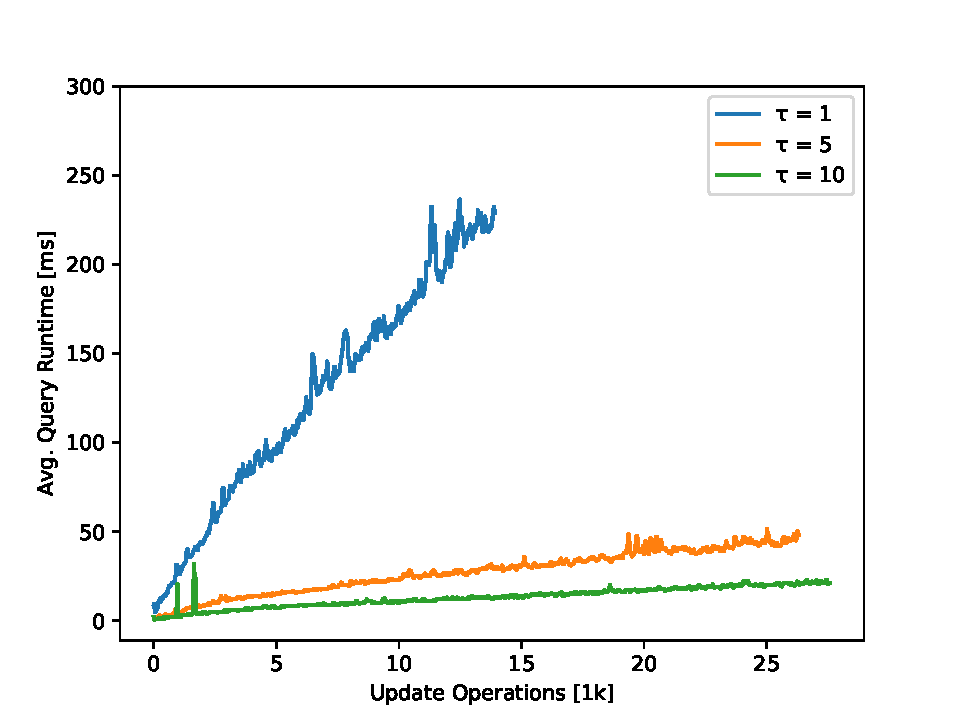
\includegraphics[width=8cm]{query_runtime_taus_synthetic}
    %\caption{}
    %\label{fig:query_runtime_taus_synthetic}
  %\end{subfigure}
  %\begin{subfigure}{0.49\linewidth}
    %\centering
    %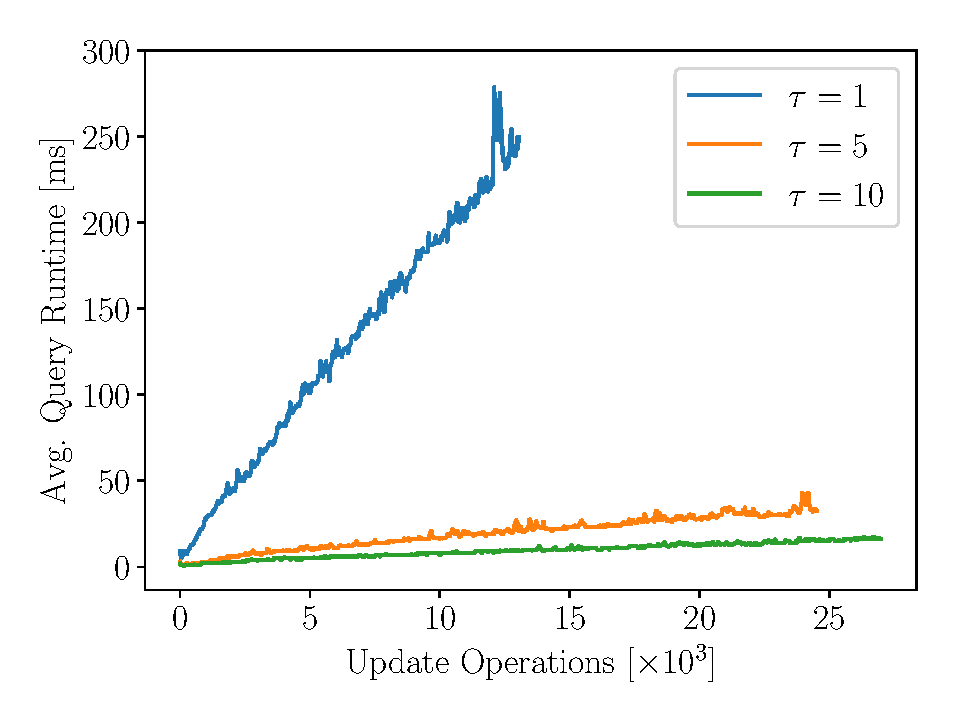
\includegraphics[width=8cm]{query_runtime_taus_real}
    %\caption{}
    %\label{fig:query_runtime_taus_real}
  %\end{subfigure}
  %\caption{Query Runtime over update operations with threshold $\tau \in \{1,5,10\}$ }
%\end{figure}

%\begin{figure}[h]
  %\centering
  %\begin{subfigure}{0.49\linewidth}
    %\centering
    %Synthetic
  %\end{subfigure}
  %\begin{subfigure}{0.49\linewidth}
    %\centering
    %Real-World
  %\end{subfigure}
  %\begin{subfigure}{0.49\linewidth}
    %\centering
    %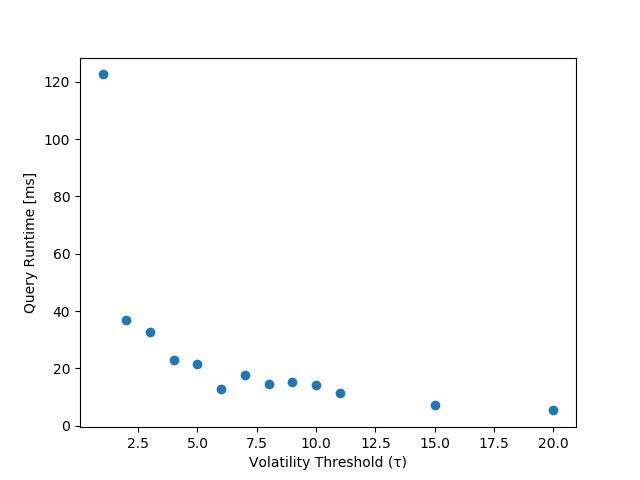
\includegraphics[width=8cm]{tau_query_runtime_synthetic}
    %\caption{}
    %\label{fig:tau_query_runtime_synthetic}
  %\end{subfigure}
  %\begin{subfigure}{0.49\linewidth}
    %\centering
    %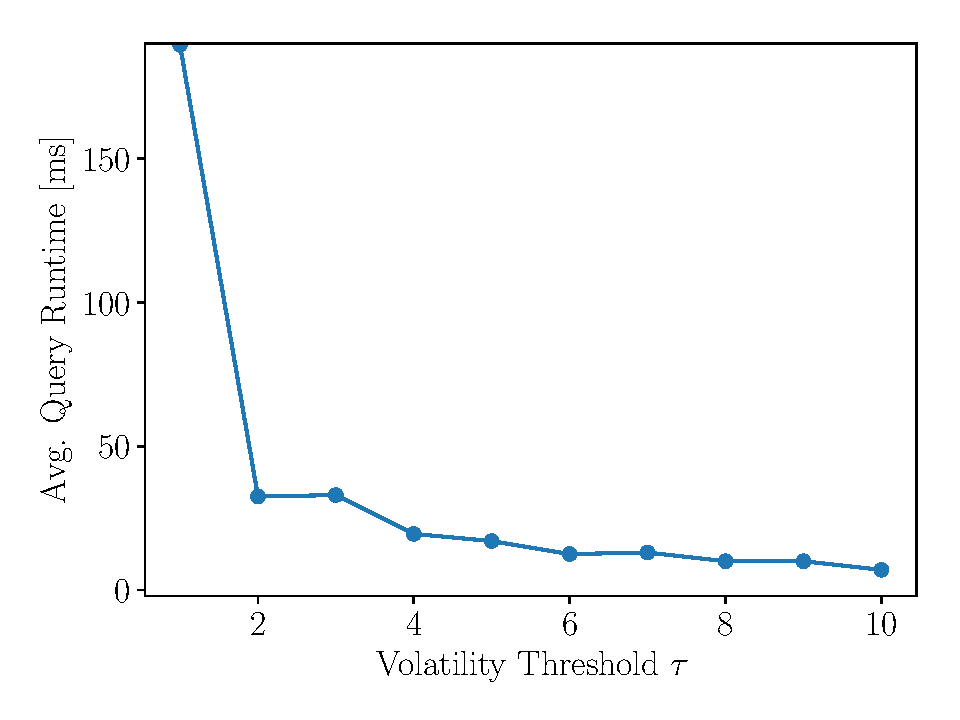
\includegraphics[width=8cm]{tau_query_runtime_real}
    %\caption{}
    %\label{fig:tau_query_runtime_real}
  %\end{subfigure}
%\caption{Query Runtime over volatility threshold $\tau$}
%\end{figure}

%We conduct the experiment under a varying volatility threshold. 
%\Cref{fig:query_runtime_taus_synthetic,fig:query_runtime_taus_real} show
%thresholds $\tau \in \{1,5,10\}$ affecting query runtime
%over update operations. We observe a decrease in query runtime
%while increasing threshold $\tau$.
%A lower volatility threshold increases the likelihood of a node
%becoming volatile. The amount of volatile nodes also affect the number of
%unproductive nodes, since volatile nodes eventually stop being frequently
%updated and become unproductive. The increase in unproductive nodes in the index
%directly affects query runtime because Oak has to traverse these nodes during
%query execution.

%\Cref{fig:tau_query_runtime_synthetic,fig:tau_query_runtime_real} compare query
%runtime over a range of thresholds. The values picked correspond to
%the query runtime after $10^4$ update operations.
%We observe a power law relationship between threshold $\tau$ and average query
%runtime. As explained above, a lower threshold increases the number of volatile
%and consequently also the number of unproductive nodes. More unproductive nodes
%do increase the query runtime. We believe the power law relationship is
%explained by the workload's skew. 

\begin{figure}[h]
  \centering
   \begin{subfigure}{0.49\linewidth}
    \centering
    \caption{Synthetic}
    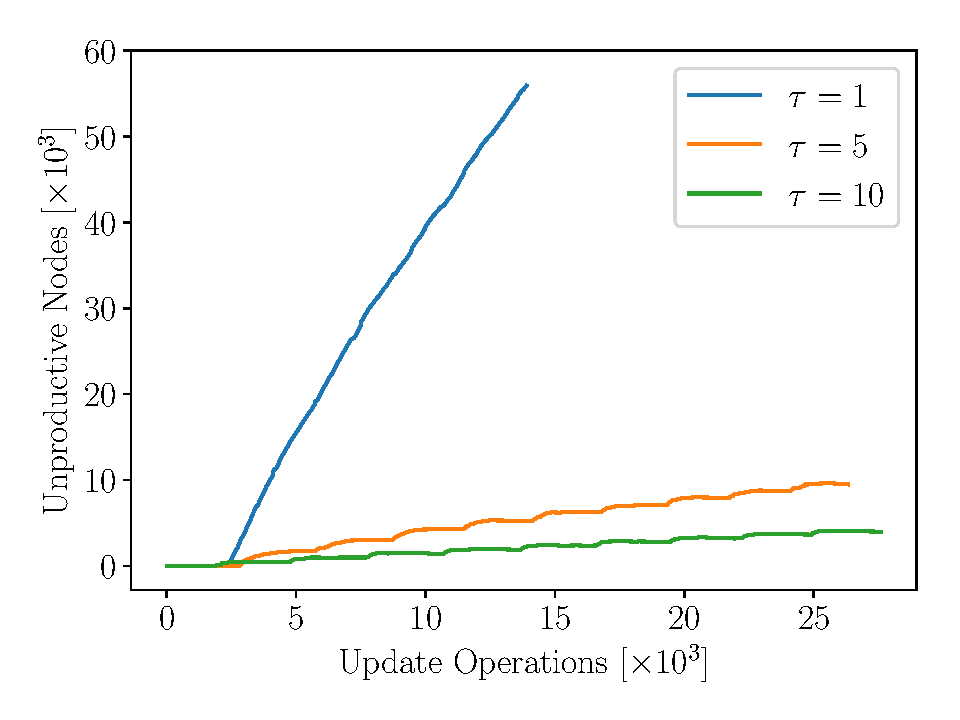
\includegraphics[width=8cm]{trav_unprod_nodes_taus_synthetic}
    \label{fig:trav_unprod_nodes_taus_synthetic}
  \end{subfigure}
  \begin{subfigure}{0.49\linewidth}
    \centering
    \caption{Real-World}
    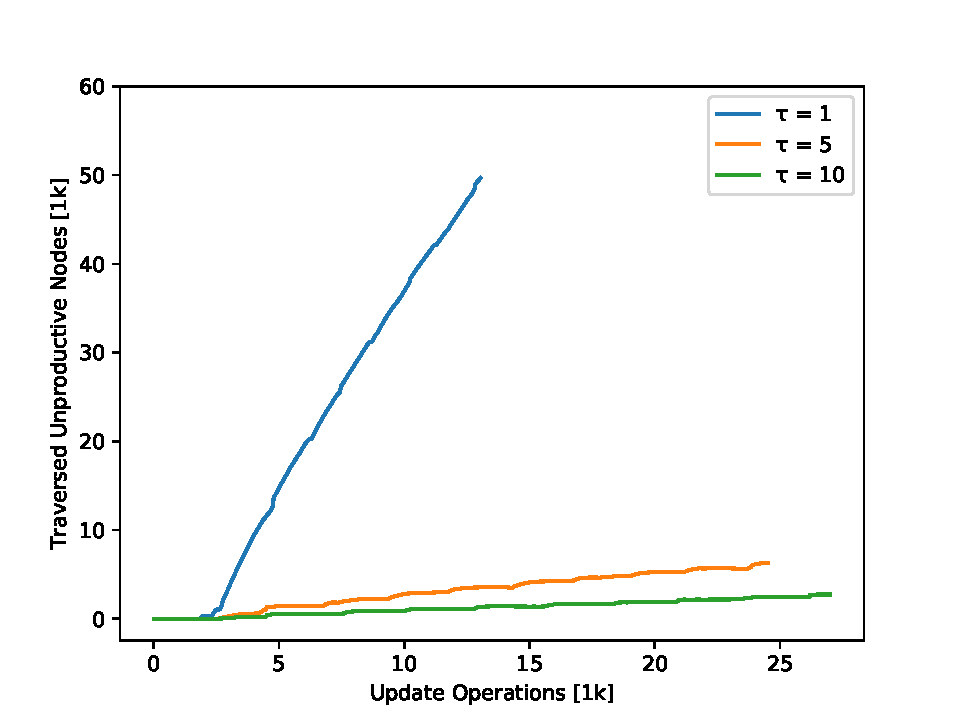
\includegraphics[width=8cm]{trav_unprod_nodes_taus_real}
    \label{fig:trav_unprod_nodes_taus_real}
  \end{subfigure}
  \vspace{-0.5cm}
  \caption{Unproductive Nodes over update operations with threshold $\tau \in \{1,5,10\}$.}
\end{figure}

\begin{figure}[h]
  \centering
  \begin{subfigure}{0.49\linewidth}
    \centering
    \caption{Synthetic}
    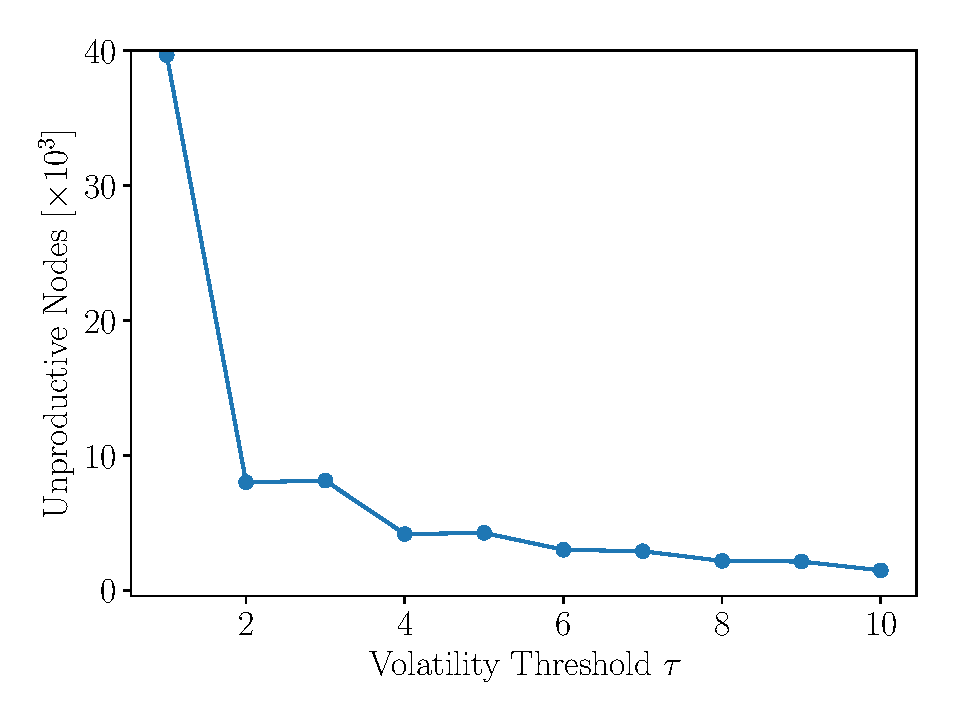
\includegraphics[width=8cm]{tau_unprod_nodes_synthetic}
    \label{fig:tau_unprod_nodes_synthetic}
  \end{subfigure}
  \begin{subfigure}{0.49\linewidth}
    \centering
    \caption{Real-World}
    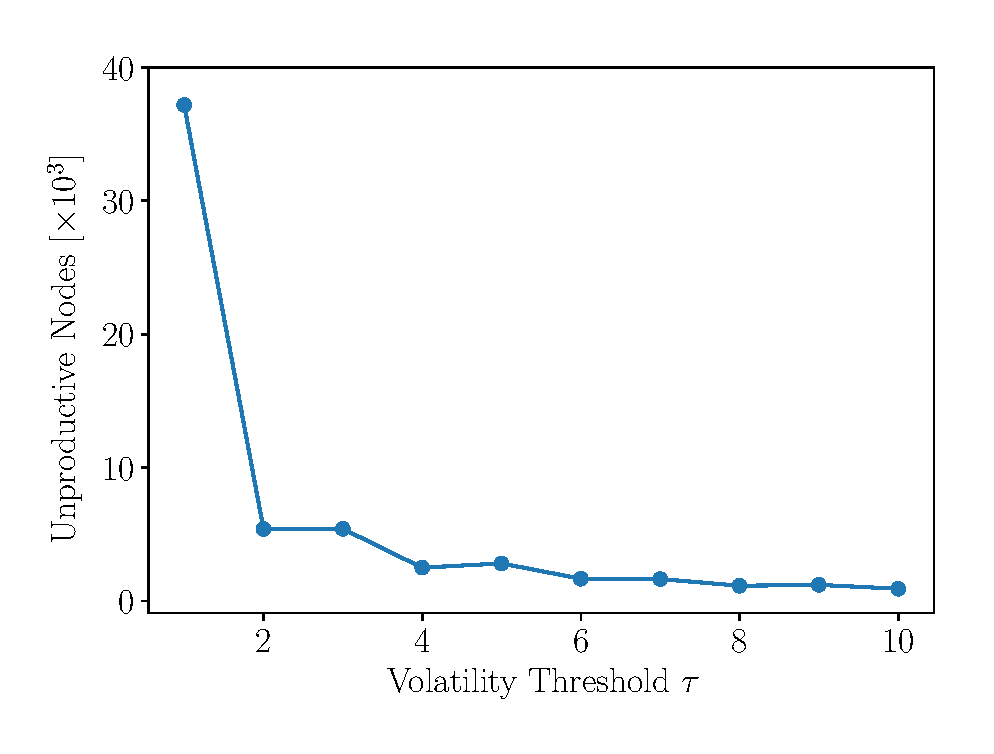
\includegraphics[width=8cm]{tau_unprod_nodes_real}
    \label{fig:tau_unprod_nodes_real}
  \end{subfigure}
  \vspace{-0.5cm}
  \caption{Unproductive Nodes over volatility threshold $\tau$.}
\end{figure}


\Cref{fig:trav_unprod_nodes_taus_synthetic,fig:trav_unprod_nodes_taus_real}
show the increase in unproductive index nodes for different
thresholds $\tau \in \{1,5,10\}$ over the course of a five minute experiment.
We observe lower thresholds $\tau$ yielding a steeper slope.
A lower volatility threshold increases the likelihood of a node
becoming volatile. The amount of volatile nodes also affect the number of
unproductive nodes, since volatile nodes eventually stop being frequently
updated when the workload changes and become unproductive. 
The increase in unproductive nodes in the index
also affects query runtime because Oak has to traverse these nodes during
query execution.

The Figures show that unproductive nodes increase linearly as update operations
increase. We expect the increase to be sublinear for longer experiments.
The number of traversed unproductive nodes is upper-bounded by the number 
of content nodes.
This is the case, because the index subtree for a given property-value pair
(e.g. pub = now) can not have
more nodes than the content subtree, because the index subtree is a subset
of the content subtree.
As time passes by, the index becomes more static (\Cref{sec:query-runtime}), 
more volatile/unproductive
index nodes are retained, less nodes are pruned. As a result, fewer nodes
become volatile. Eventually, we will reach the upper bound.

\Cref{fig:tau_unprod_nodes_synthetic,fig:tau_unprod_nodes_real} compare the
number of traversed unproductive nodes during query execution over a range of
thresholds. We observe a decrease in unproductive nodes while increasing
threshold $\tau$. 
As suggested earlier, a lower volatility threshold
increases the amount of volatile nodes in the index and consequently also
increases the number of unproductive nodes. 

We see the two variables sharing a power law relationship. We believe the
workload's skew to be responsible for the power law relationship. 
The query executor has to traverse $5k$ unproductive index nodes when Oak has a
threshold of $\tau = 5$. By increasing the threshold to $\tau = 6$, the average
number of traversed unproductive nodes does not decrease significantly because
of the Zipf distribution's skewness. The majority of update operations are executed
amongst a small subset of nodes. This explains the power law relationship
between traversed unproductive nodes and $\tau$.

At $\tau = 0$, any node drawn by the workload becomes volatile. That is why we
see so many unproductive nodes. At $\tau = 2$, we observe a sudden drop in 
unproductive nodes. That is because content nodes have to be drawn twice in order
to become unproductive, and since the workload is skewed, only a few nodes are
drawn twice. For even larger values, the function flattens out. Since the workload
is skewed, only a handful of nodes are drawn enough by the workload to become volatile.

Summarizing, all observations verify our hypotheses.
Increasing volatility threshold $\tau$ decreases the number of unproductive
nodes traversed which decreases query runtime. Increasing the volatility
threshold causes less nodes to become volatile. Since we create less volatile
nodes, we also reduce the number of unproductive nodes. Less unproductive
nodes yield lower WAPI query runtimes. 

\subsubsection{Sliding Window of Length $L$}

\label{sec:sliding-window}

The Sliding Window Length $L$ determines the length of the recent workload that WAPI
considers to compute an index node's volatility count (cf. \Cref{def:volatile_node}).
Greater values of $L$
allow WAPI to count more updates and therefore increase the chances of a node
becoming volatile. In this section, we study
the effect of the sliding window on the number unproductive nodes.

We hypothesize that an increase in $L$ yields an increase to the number of
traversed unproductive nodes during query execution. If $L$ increases, it is
more likely for a node to become volatile, since more updates are considered
towards the volatility count.
Having more volatile nodes should imply an increase in unproductive nodes and
consequently also query runtime.

% \begin{shaded}
%   \begin{itemize}
%   \item[$H_5$:] An increase in $L$ yields an increase to WAPI's query runtime
%     under a CMS workload. 
%   \item[$H_6$:] An increase in $L$ should increase the number of unproductive
%     nodes WAPI traverses during query execution under a CMS workload.
%   \end{itemize}
% \end{shaded}

% We conduct our experiment with a varying sliding window length and present our
% observations below.

%\begin{figure}[h]
  %\centering
  %\begin{subfigure}{0.49\linewidth}
    %\centering
    %Synthetic
  %\end{subfigure}
  %\begin{subfigure}{0.49\linewidth}
    %\centering
    %Real-World
  %\end{subfigure}
  %\begin{subfigure}{0.49\linewidth}
    %\centering
    %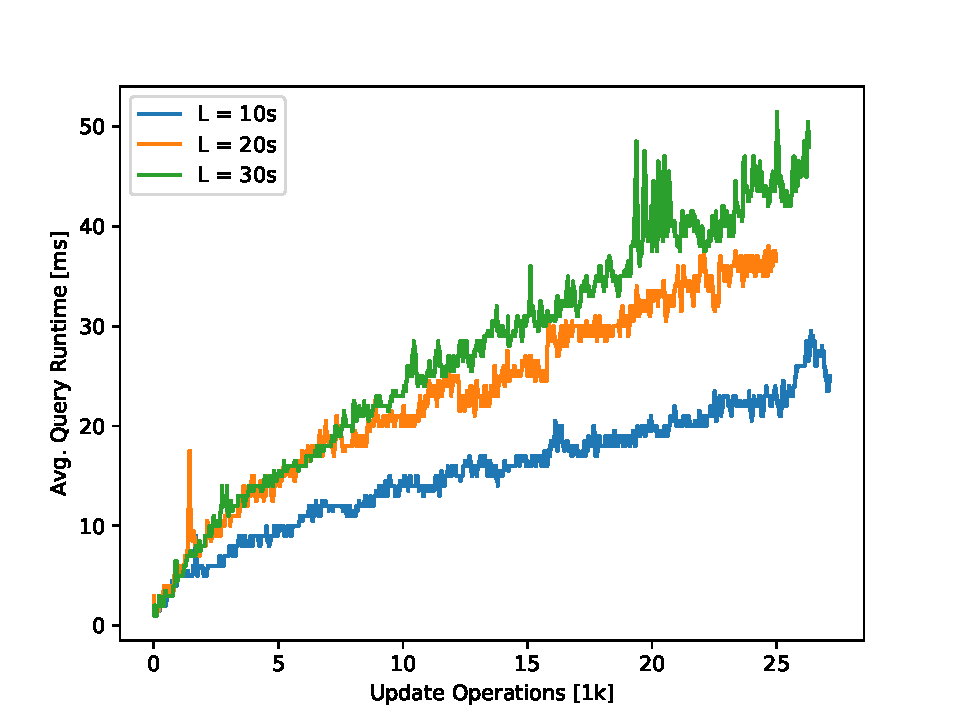
\includegraphics[width=8cm]{query_runtime_Ls_synthetic}
    %\caption{}
    %\label{fig:query_runtime_Ls_synthetic}
  %\end{subfigure}
  %\begin{subfigure}{0.49\linewidth}
    %\centering
    %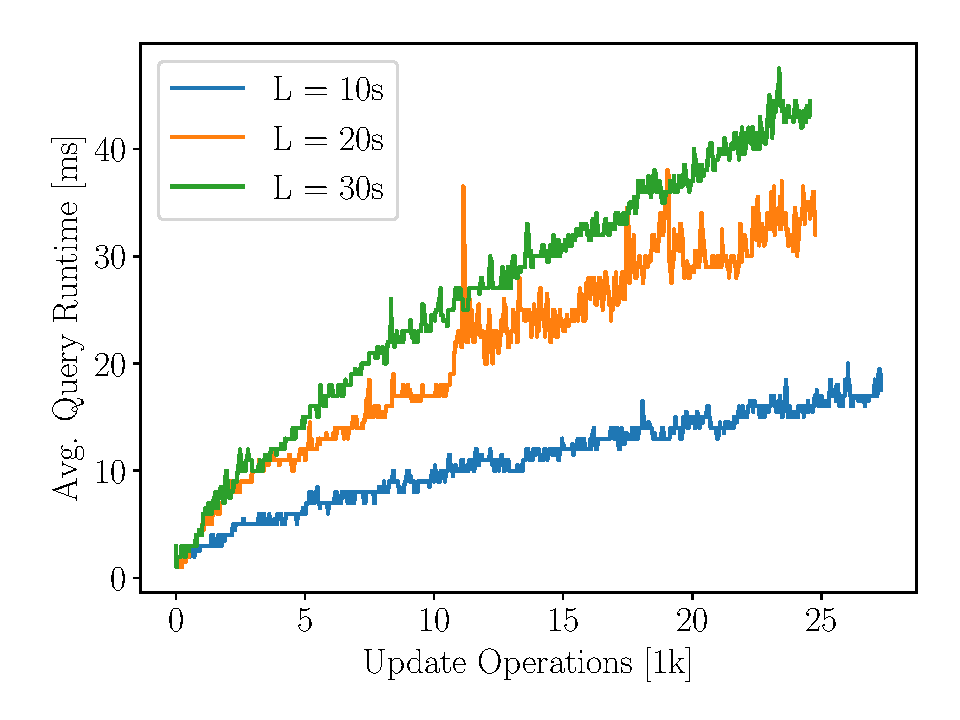
\includegraphics[width=8cm]{query_runtime_Ls_real}
    %\caption{}
    %\label{fig:query_runtime_Ls_real}
  %\end{subfigure}
  %\caption{Query Runtime over update operations with sliding window 
  %of length $L \in \{10s,20s,30s\}$ }
%\end{figure}

%\begin{figure}[h]
  %\centering
  %\begin{subfigure}{0.49\linewidth}
    %\centering
    %Synthetic
  %\end{subfigure}
  %\begin{subfigure}{0.49\linewidth}
    %\centering
    %Real-World
  %\end{subfigure}
  %\begin{subfigure}{0.49\linewidth}
    %\centering
    %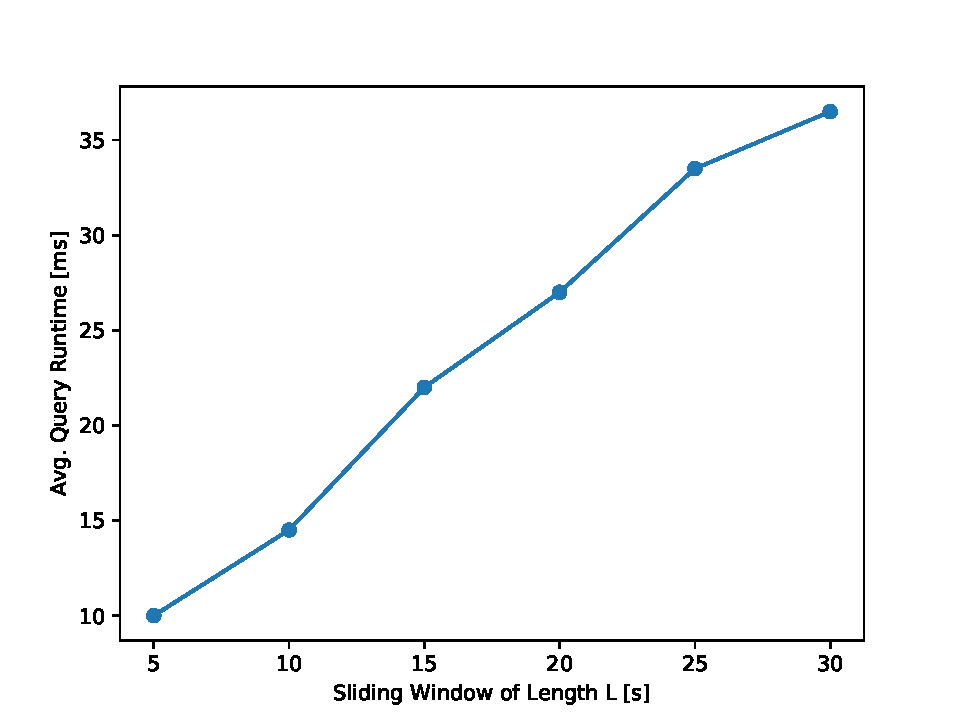
\includegraphics[width=8cm]{L_query_runtime_synthetic}
    %\caption{}
    %\label{fig:L_query_runtime_synthetic}
  %\end{subfigure}
  %\begin{subfigure}{0.49\linewidth}
    %\centering
    %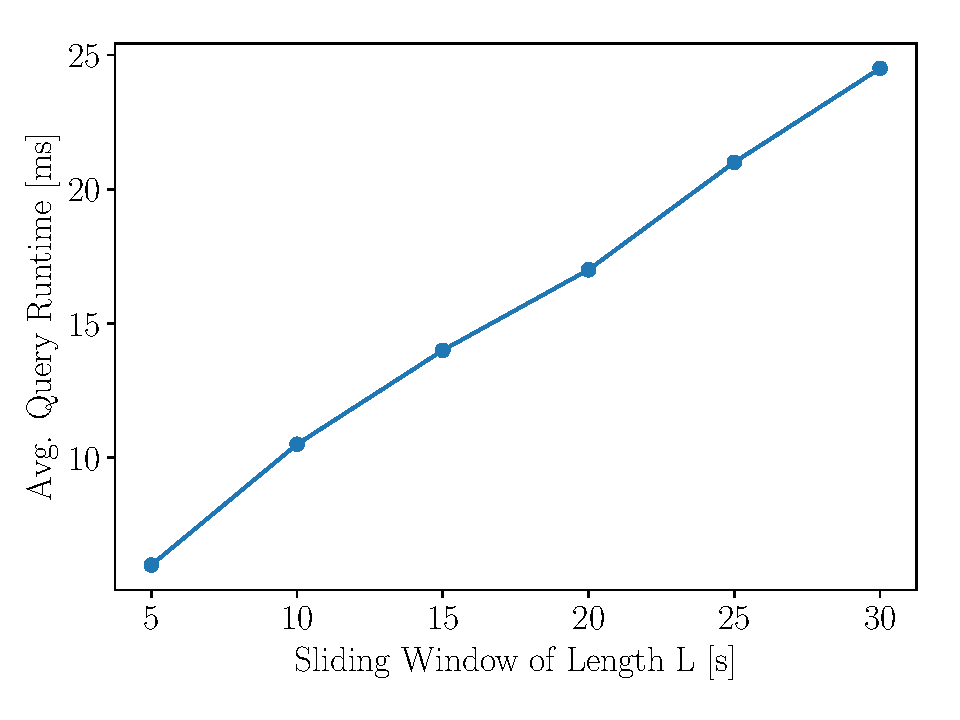
\includegraphics[width=8cm]{L_query_runtime_real}
    %\caption{}
    %\label{fig:L_query_runtime_real}
  %\end{subfigure}
  %\caption{Query Runtime over sliding window length $L$}
%\end{figure}


%\Cref{fig:query_runtime_Ls_synthetic,fig:query_runtime_Ls_real} show WAPI's average
%query runtime over update operations with sliding window of length $L \in \{10, 20,
%30\}$ seconds.
%\Cref{fig:L_query_runtime_synthetic,fig:L_query_runtime_real} depict query
%runtime with respect to the sliding window. 
%We see queries being executed by a WAPI with a greater $L$ to have greater
%runtimes on average. By increasing the sliding
%window, we increase the likelihood of a node becoming volatile because the WAPI
%counts more updates towards the volatility count. As a result, the number of
%unproductive nodes increases as well. Since the WAPI has to traverse
%more unproductive nodes during query execution, the query runtime increases.

\begin{figure}[h]
  \centering
  \begin{subfigure}{0.49\linewidth}
    \centering
    \caption{Synthetic}
    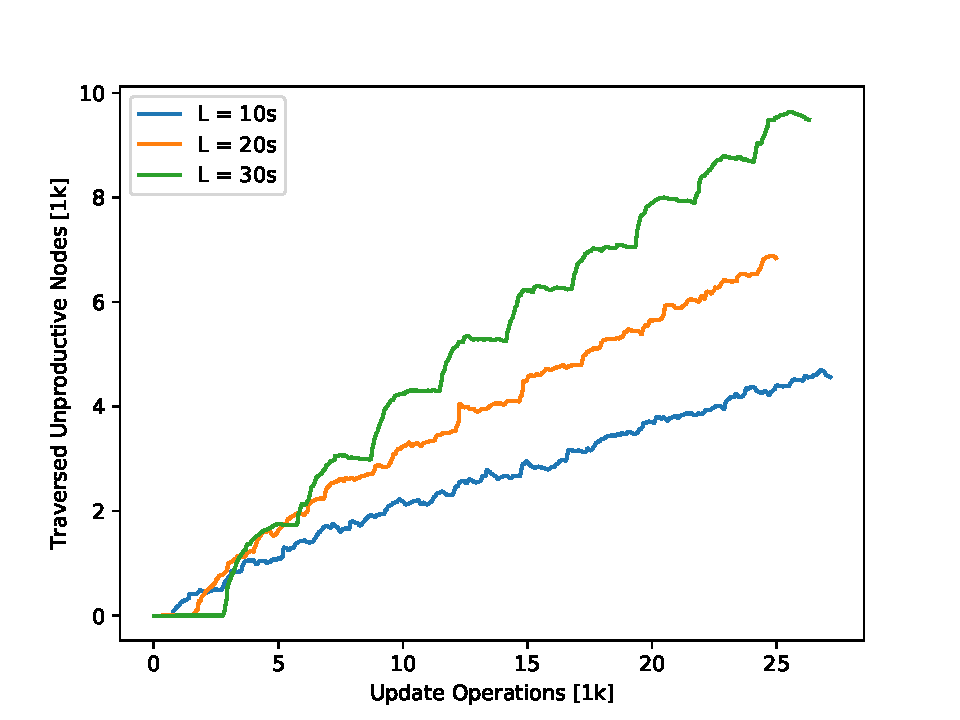
\includegraphics[width=8cm]{trav_unprod_nodes_Ls_synthetic}
    \label{fig:trav_unprod_nodes_Ls_synthetic}
  \end{subfigure}
  \begin{subfigure}{0.49\linewidth}
    \centering
    \caption{Real-World}
    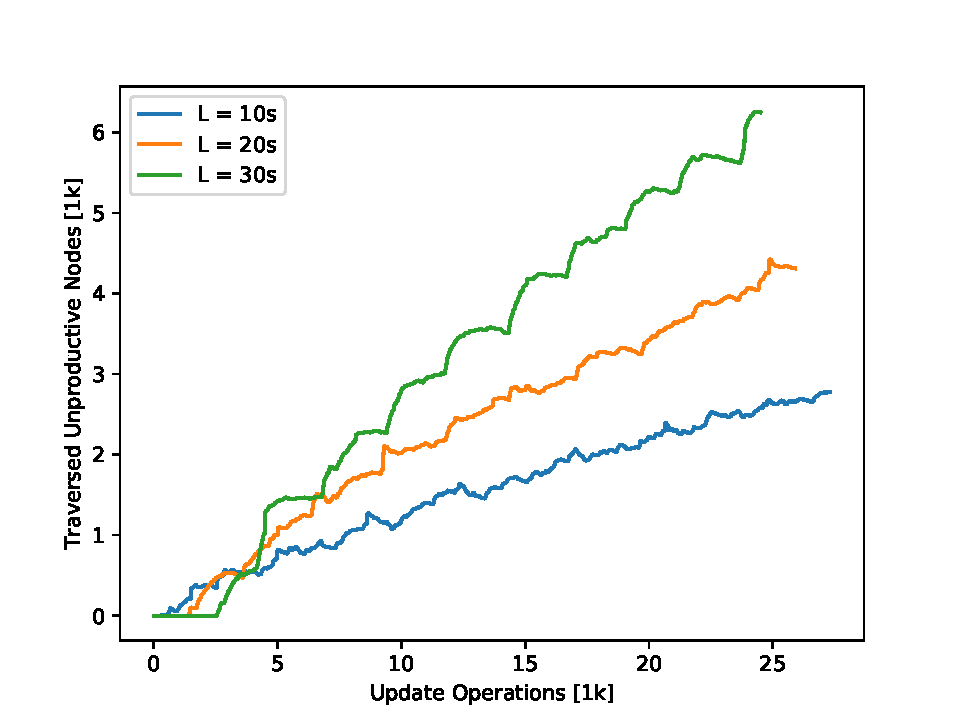
\includegraphics[width=8cm]{trav_unprod_nodes_Ls_real}
    \label{fig:trav_unprod_nodes_Ls_real}
  \end{subfigure}
  \vspace{-0.5cm}
  \caption{Traversed Unproductive Nodes over update operations with sliding 
  window of length $L \in \{10s,20s,30s\}$.}
\end{figure}

\begin{figure}[h]
  \centering
  \begin{subfigure}{0.49\linewidth}
    \centering
    \caption{Synthetic}
    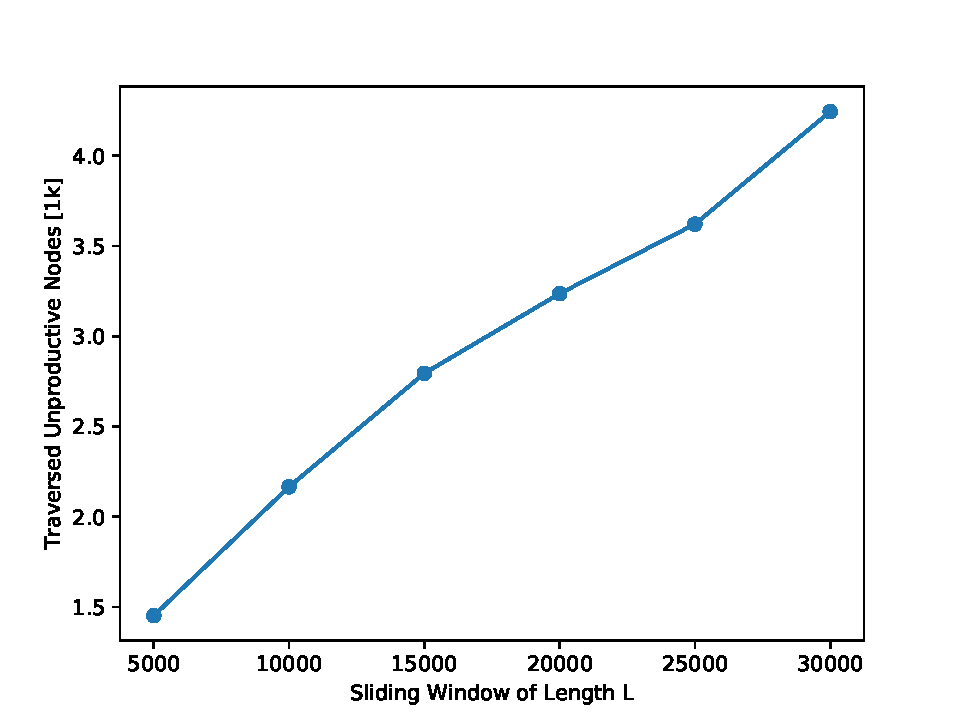
\includegraphics[width=8cm]{L_unprod_nodes_synthetic}
    \label{fig:L_trav_unprod_nodes_synthetic}
  \end{subfigure}
  \begin{subfigure}{0.49\linewidth}
    \centering
    \caption{Real-World}
    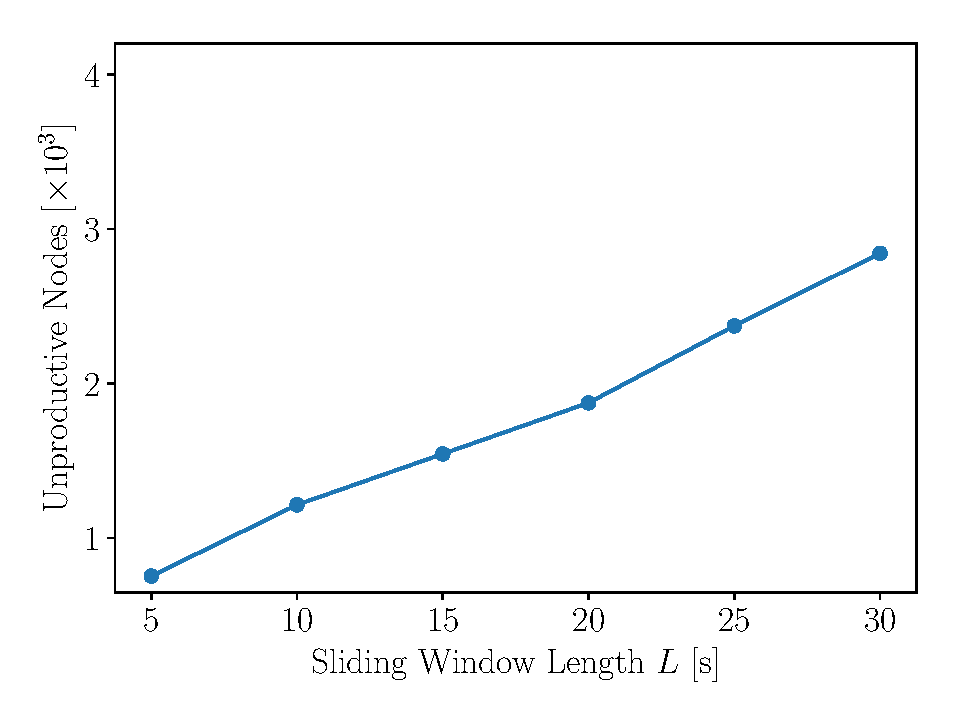
\includegraphics[width=8cm]{L_unprod_nodes_real}
    \label{fig:L_trav_unprod_nodes_real}
  \end{subfigure}
  \vspace{-0.5cm}
  \caption{Traversed Unproductive Nodes over sliding window length $L$.}
\end{figure}

\Cref{fig:trav_unprod_nodes_Ls_synthetic,fig:trav_unprod_nodes_Ls_real} visualize
the number of unproductive nodes WAPI traverses during query execution for
three distinct lengths $L \in \{10s,20s,30s\}$ of the sliding window with
respect to update operations. As expected, the number of unproductive nodes
increases the fastest for the longest sliding window length ($L = 30s$).
In the long term,
the number of unproductive nodes increases sublinearly with respect to time.
We explained earlier that as time passes, the index becomes more static
and the number of unproductive nodes converges towards the upper bound
set by the number of content nodes.

\Cref{fig:L_trav_unprod_nodes_synthetic,fig:L_trav_unprod_nodes_real} show the
number of unproductive nodes the query executor has to traverse with respect
to the sliding window length $L$. Greater sliding window lengths 
cause a sublinear increase to the number of unproductive nodes traversed 
by WAPI during query execution. Since the index becomes more static 
as explained earlier, the function converges towards the upper bound. 
The Figures seem to suggest a linear relationship
between the two variables. That is because the number of content nodes is greater
by two orders of magnitude compared to the number of unproductive nodes we can
produce during the entire five-minute experiment. We expect to see the function 
converge if we run the experiment for a significantly longer duration of time.

Concluding, we see sliding window of length $L$ to be affecting the rate of growth of
unproductive nodes.
Increasing $L$ does increase the likelihood of an index node to become volatile
and later unproductive.

\subsubsection{Workload Skew $s$}

\label{sec:skew}

One of the key characteristics of the CMS Workload is skewness, as mentioned in 
\Cref{sec:application_scenario}. A small subset of nodes is frequently updated,
whereas the rest of the nodes is not. We refer to the set of content nodes
which are frequently drawn by the skewed workload as \textit{hotspot}.
Nodes inside the hotspot most likely become volatile and later on unproductive.
We use the Zipf distribution to model a skewed workload (\Cref{sec:workload}).
If skew $s$ increases, the hotspot becomes smaller 
but the hotspot's member nodes are drawn more frequent.

\begin{figure}[h]
  \centering
  \begin{subfigure}{0.30\textwidth}
    \centering
    \scriptsize
    \begin{forest}
      [,circle,draw,fill=YellowOrange
      [,circle,draw,fill=YellowOrange
      [,circle,draw,fill=YellowOrange
      ]
      [,circle,draw,fill=YellowOrange
      [,circle,draw,fill=YellowOrange]
      [,phantom]
      ]
      ]
      [,circle,draw,fill=YellowOrange
      [,phantom]
      [,circle,draw,fill=YellowOrange
      [,circle,draw,fill=YellowOrange]
      [,circle,draw,fill=YellowOrange]
      ]
      ]
      ]
    \end{forest}

    No skew ($s=0$)
  \end{subfigure}
  \begin{subfigure}{0.30\textwidth}
    \centering
    \scriptsize
    \begin{forest}
      [,circle,draw,fill=Yellow
      [,circle,draw,fill=Yellow
      [,circle,draw,fill=Yellow
      ]
      [,circle,draw,fill=Yellow
      [,circle,draw,fill=Orange]
      [,phantom]
      ]
      ]
      [,circle,draw,fill=Orange
      [,phantom]
      [,circle,draw,fill=Yellow
      [,circle,draw,fill=Red]
      [,circle,draw,fill=Orange]
      ]
      ]
      ]
    \end{forest}
  
    Normal skew ($s=1$)
  \end{subfigure}
  \begin{subfigure}{0.30\textwidth}
    \centering
    \scriptsize
    \begin{forest}
      [,circle,draw,fill=Yellow
      [,circle,draw,fill=Yellow
      [,circle,draw,fill=Yellow
      ]
      [,circle,draw,fill=Yellow
      [,circle,draw,fill=Yellow]
      [,phantom]
      ]
      ]
      [,circle,draw,fill=Yellow
      [,phantom]
      [,circle,draw,fill=Yellow
      [,circle,draw,fill=Red]
      [,circle,draw,fill=Red]
      ]
      ]
      ]
    \end{forest}

    High skew ($s>1$)
  \end{subfigure}

  \caption[Hotspots affected by different skew values]{Hotspots affected by different skew values.
  Red shaded nodes denote frequently drawn nodes.}
  \label{fig:skew}
\end{figure}

We expect skew $s$ to affect the number of unproductive nodes WAPI traverses during
query execution. Since some nodes are updated more often, these nodes are more likely
to become volatile
and also unproductive, later on. On the other hand, increasing skew $s$ also reduces
the size of the hotspot and therefore reduce
the number of volatile nodes, hence less nodes become unproductive.

\Cref{fig:skew} visualizes workloads with different skew values for the
reader's convenience. In the uniform workload, that is the workload with no skew ($s=0$),
each node is equaly likely to be drawn. The workload with skew $s=1$ has a hotspot
and nodes in the hotspot are drawn more frequent than other nodes. The workload
with high skew ($s>1$) has an even smaller hotspot but member nodes are drawn more frequent.

%\begin{figure}[h]
  %\centering
  %\begin{subfigure}{0.49\linewidth}
    %\centering
    %Synthetic
  %\end{subfigure}
  %\begin{subfigure}{0.49\linewidth}
    %\centering
    %Real-World
  %\end{subfigure}
  %\begin{subfigure}{0.49\linewidth}
    %\centering
    %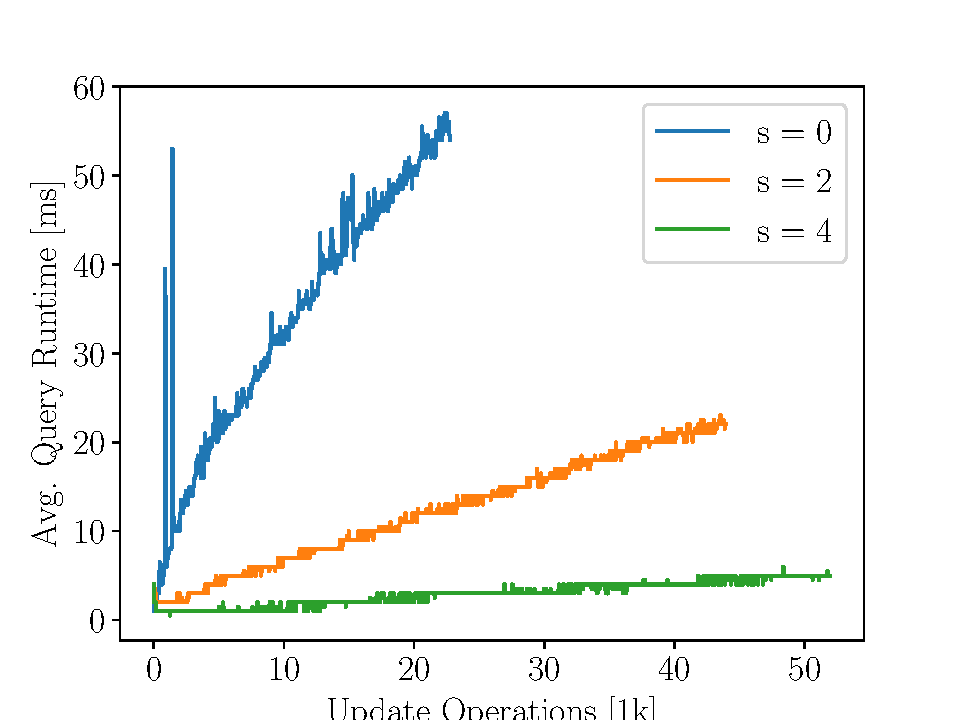
\includegraphics[width=8cm]{query_runtime_skews_synthetic}
    %\caption{}
    %\label{fig:query_runtime_skews_synthetic}
  %\end{subfigure}
  %\begin{subfigure}{0.49\linewidth}
    %\centering
    %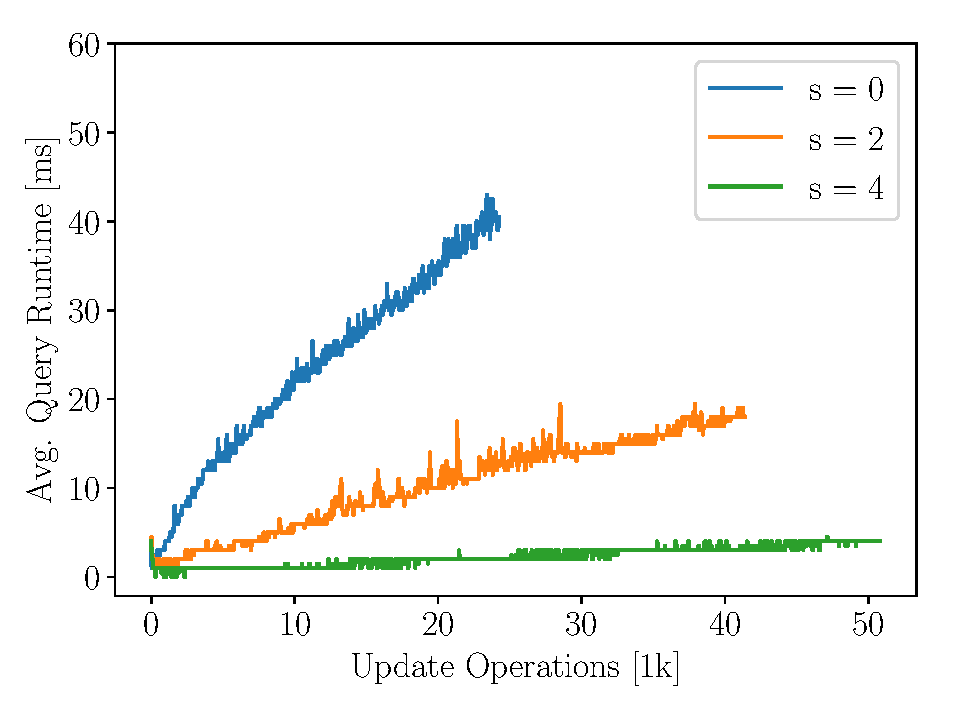
\includegraphics[width=8cm]{query_runtime_skews_real}
    %\caption{}
    %\label{fig:query_runtime_skews_real}
  %\end{subfigure}
  %\caption{Query Runtime over update operations with skew $s \in \{0,2,4\}$ }
%\end{figure}

%\begin{figure}[h]
  %\centering
  %\begin{subfigure}{0.49\linewidth}
    %\centering
    %Synthetic
  %\end{subfigure}
  %\begin{subfigure}{0.49\linewidth}
    %\centering
    %Real-World
  %\end{subfigure}
  %\begin{subfigure}{0.49\linewidth}
    %\centering
    %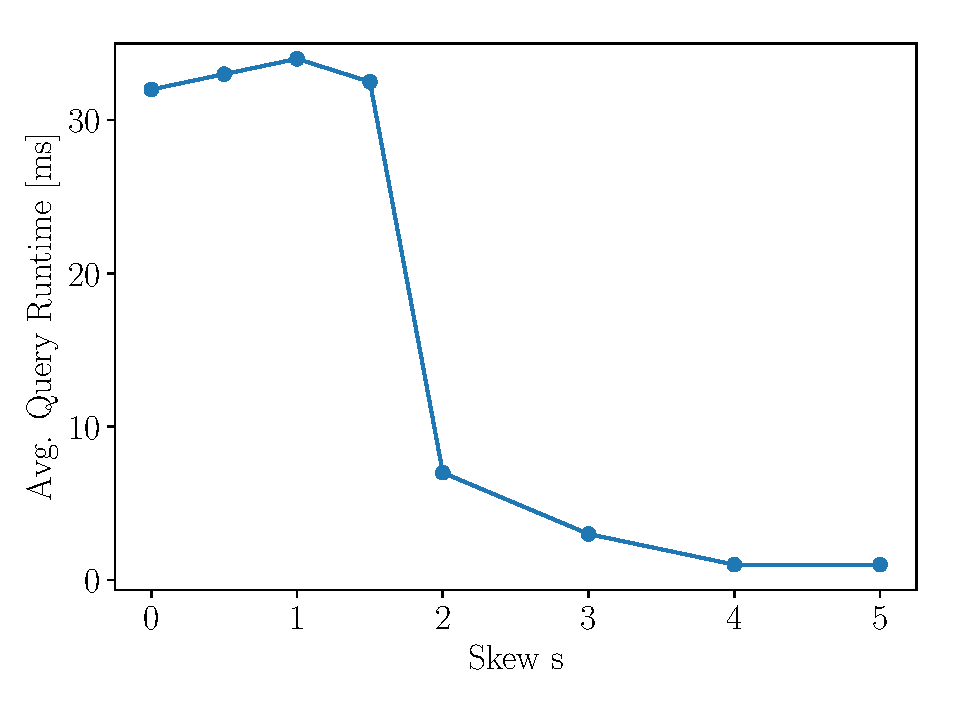
\includegraphics[width=8cm]{skew_query_runtime_synthetic}
    %\caption{}
    %\label{fig:skew_query_runtime_synthetic}
  %\end{subfigure}
  %\begin{subfigure}{0.49\linewidth}
    %\centering
    %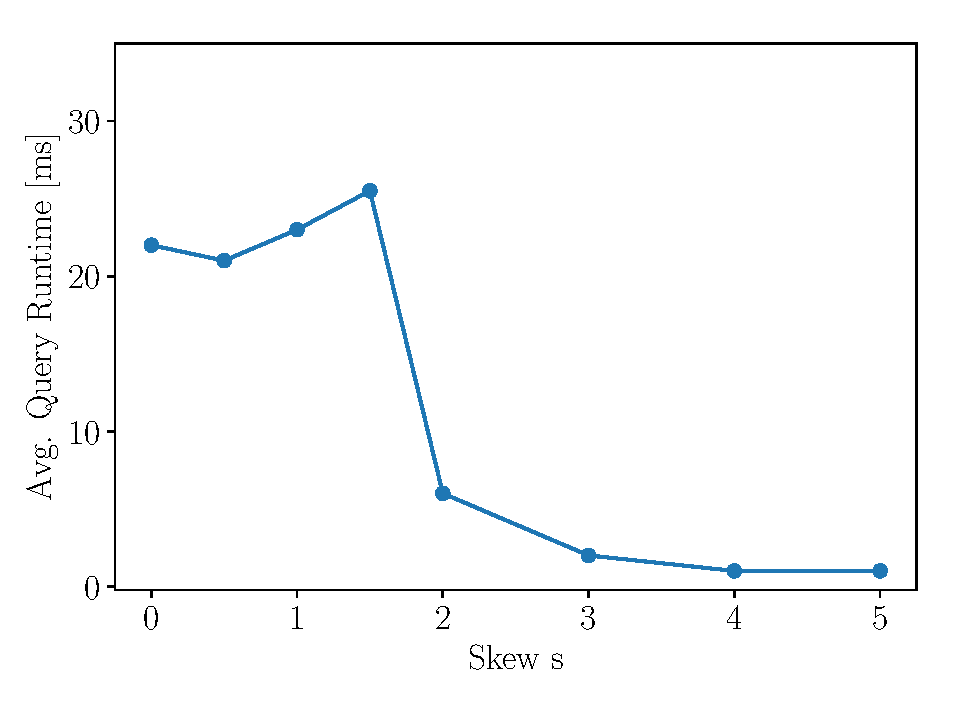
\includegraphics[width=8cm]{skew_query_runtime_real}
    %\caption{}
    %\label{fig:skew_query_runtime_real}
  %\end{subfigure}
%\caption{Query Runtime over skew $s$}
%\end{figure}

\begin{figure}[h]
  \centering
  \begin{subfigure}{0.49\linewidth}
    \centering
    \caption{Synthetic}
    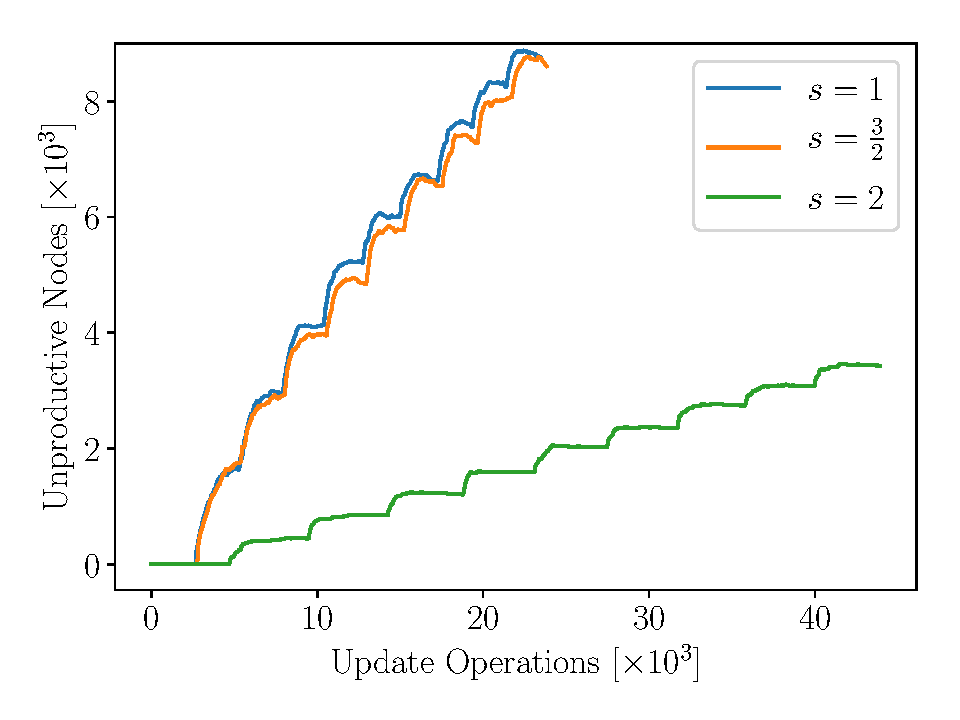
\includegraphics[width=8cm]{trav_unprod_nodes_skews_synthetic}
    \label{fig:trav_unprod_nodes_skews_synthetic}
  \end{subfigure}
  \begin{subfigure}{0.49\linewidth}
    \centering
    \caption{Real-World}
    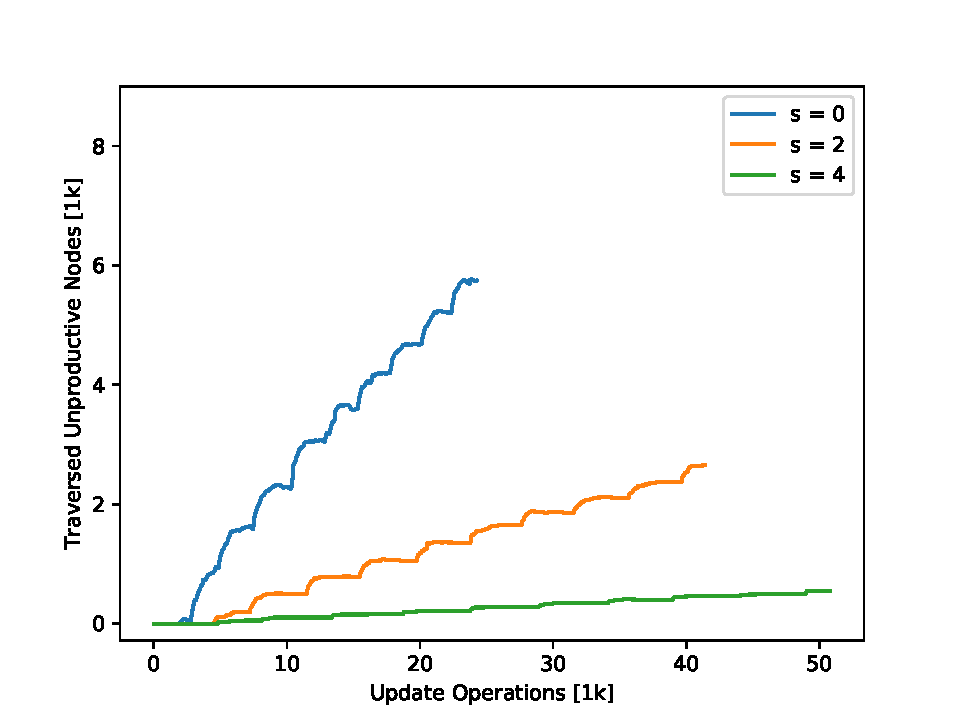
\includegraphics[width=8cm]{trav_unprod_nodes_skews_real}
    \label{fig:trav_unprod_nodes_skews_real}
  \end{subfigure}
  \vspace{-0.5cm}
  \caption{Unproductive Nodes over update operations with skew $s \in \{
  1, \frac{3}{2}, 2\}$.}
\end{figure}

\begin{figure}[h]
  \centering
  \begin{subfigure}{0.49\linewidth}
    \centering
    \caption{Synthetic}
    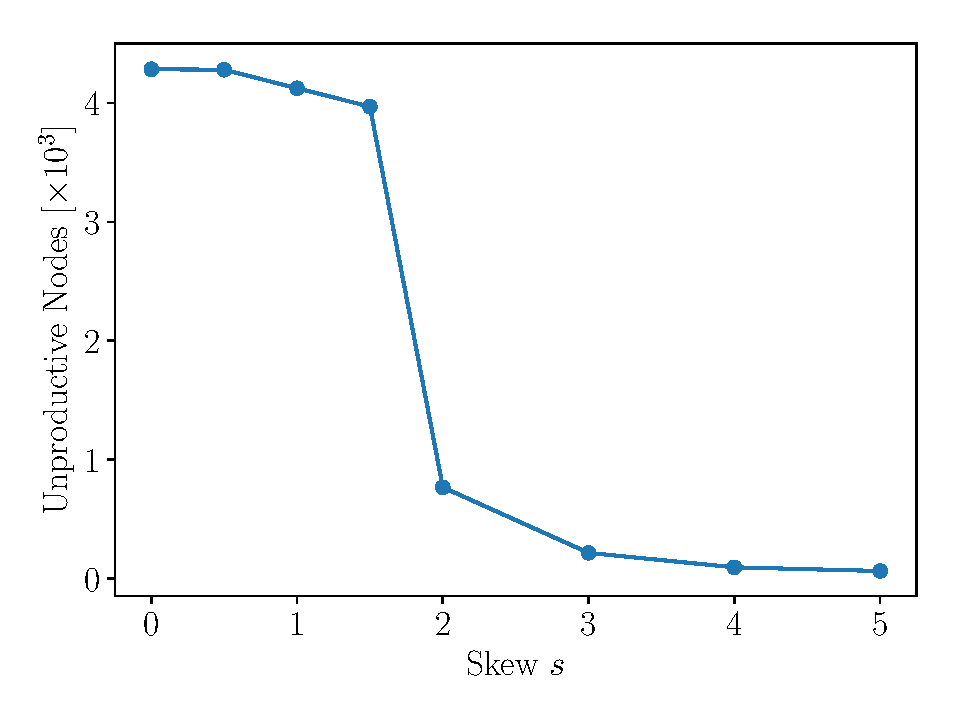
\includegraphics[width=8cm]{skew_unprod_nodes_synthetic}
    \label{fig:skew_unprod_nodes_synthetic}
  \end{subfigure}
  \begin{subfigure}{0.49\linewidth}
    \centering
    \caption{Real-World}
    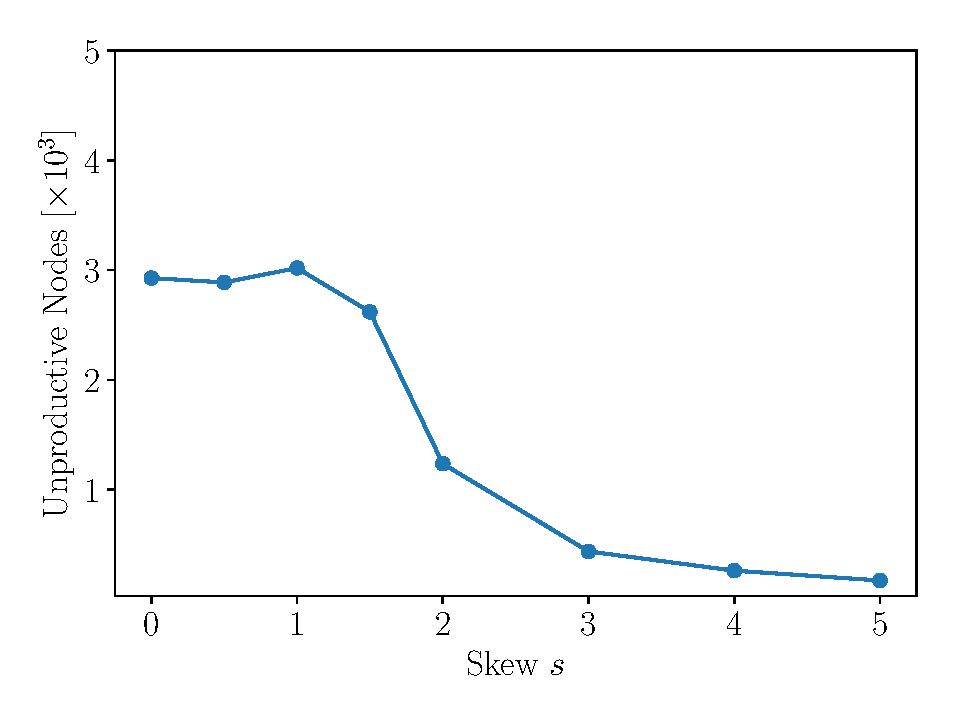
\includegraphics[width=8cm]{skew_unprod_nodes_real}
    \label{fig:skew_unprod_nodes_real}
  \end{subfigure}
  \vspace{-0.5cm}
  \caption{Unproductive Nodes over skew $s$.}
\end{figure}

\Cref{fig:trav_unprod_nodes_skews_synthetic,fig:trav_unprod_nodes_skews_real} show the number
of unproductive nodes traversed by WAPI during query execution with workloads having skew
$s \in \{1,\frac{3}{2},2\}$.  We see a smaller
skew $s$ increases the number of unproductive nodes. We believe that when increasing $s$, 
the size of the hotspot decreases and therefore the number of nodes
becoming volatile, and eventually unproductive, decreases.
We also see that a workload with $s = 1$ has barely more unproductive nodes over time
than a workload with $s = \frac{3}{2}$. We believe that if we run the experiment
significantly longer, the difference between the two workloads would be greater.

\Cref{fig:skew_unprod_nodes_synthetic,fig:skew_unprod_nodes_real} offer a more detailed
perspective by showing the traversed unproductive nodes with respect to skew $s$. We see a
sudden drop in unproductive nodes when skew is $s = 2$. 
The hotspot reaches a point where it loses a significant amount of nodes because the 
workload is so skewed. From there on, we see a sublinear rate of convergence. 
%When $s \to \infty$,
%the hotspot only has a single member which gets exclusively updated, as proven below:

%\vspace{-0.5cm}

%\begin{align*}
    %\lim_{s \to \infty} Zipf(k,N,s)
    %& = \lim_{s \to \infty} \frac{ \frac{1}{k^s} }{\sum^{N}_{i=1} \frac{1}{i^s}}
    %= \lim_{s \to \infty} \frac{ \frac{1}{k^s} }{\frac{1}{1^s} + \sum^{N}_{i=2} \frac{1}{i^s}} \\
    %& = \frac{\frac{1}{k^\infty}}{ \frac{1}{1^\infty} + \sum^{N}_{i=2} \frac{1}{i^\infty}}
    %= \frac{\frac{1}{k^\infty}}{ \frac{1}{1^\infty} + \sum^{N}_{i=2} \frac{1}{\infty}} \\
    %& = \frac{\frac{1}{k^\infty}}{ \frac{1}{1} + \sum^{N}_{i=2} 0}
    %= \frac{\frac{1}{k^\infty}}{1 + 0} \\
    %& = \frac{1}{k^\infty} \\
    %\text{for}\ k = 1 : \quad \frac{1}{k^\infty} & = \frac{1}{1^\infty} = 1 \\
    %\text{for}\ k > 1 : \quad \frac{1}{k^\infty} & = \frac{1}{\infty} = 0
%\end{align*}

%No other nodes besides the node with $k = 1$ gets drawn from the Zipf distribution 
%when $s \to \infty$.

%We also see another interesting phenomenon. Comparing the synthetic to the real-world
%dataset, we see the number of unproductive nodes decrease in the interval
%$s \in [0,1]$, whilst it increases during the same interval in the real-world dataset.
%The synthetic dataset produces the most unproductive nodes with a uniform workload ($s = 0$).
%We conjecture that the low sparsity in the synthetic dataset is responsible for the
%observed phenomenon.

\subsubsection{Update to Query Ratio}

\label{sec:update-query-ratio}

One of our initial assumptions was that Oak's workload is update heavy, amongst others.
To emphasize the implications of such an update heavy workload, we conduct the following
experiment. Oak is benchmarked with different update to query ratios,
that is the number of updates executed between two consecutive queries,
in order to show the effect of such a workload
on unproductive nodes. 

\begin{figure}[h]
  \centering
  \begin{subfigure}{0.49\linewidth}
    \centering
    \caption{Synthetic}
    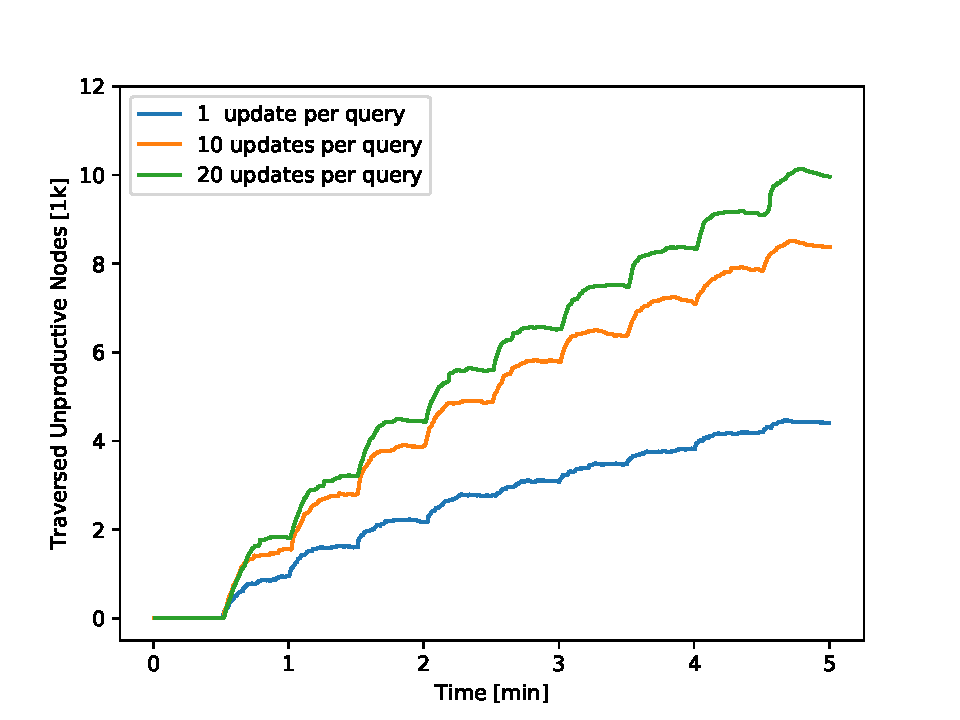
\includegraphics[width=8cm]{trav_unprod_nodes_upt_synthetic}
    \label{fig:trav_unprod_nodes_upt_synthetic}
  \end{subfigure}
  \begin{subfigure}{0.49\linewidth}
    \centering
    \caption{Real-World}
    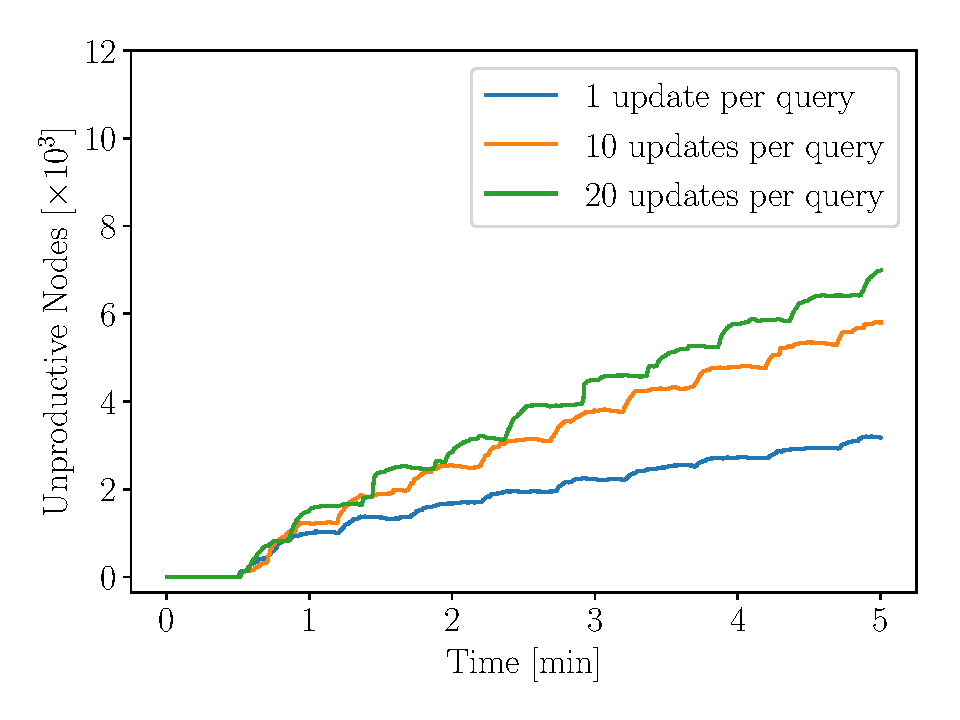
\includegraphics[width=8cm]{trav_unprod_nodes_upt_real}
    \label{fig:trav_unprod_nodes_upt_real}
  \end{subfigure}
  \vspace{-0.5cm}
  \caption{Traversed Unproductive Nodes over time for 1, 10 and 20 updates per query.}
\end{figure}


\Cref{fig:trav_unprod_nodes_upt_synthetic,fig:trav_unprod_nodes_upt_real} show
the number of traversed unproductive nodes over time. We run the simulation for
three update to query ratios: 1, 10 and 20 updates per query. An increase
in updates yields an increase in traversed unproductive nodes, an observation
depicted in \Cref{fig:upt_unprod_nodes_synthetic,fig:upt_unprod_nodes_real}, too.
The latter Figures show the number of traversed unproductive nodes over updates
per query.
A node becomes volatile if it is updated $\tau$ times during a sliding window of length $L$.
If we increase the number of updates, the node is more likely to become volatile.
If the number of volatile nodes increases, there is an increase in unproductive nodes, too,
as shown before.

\begin{figure}[h]
  \centering
  \begin{subfigure}{0.49\linewidth}
    \centering
    \caption{Synthetic}
    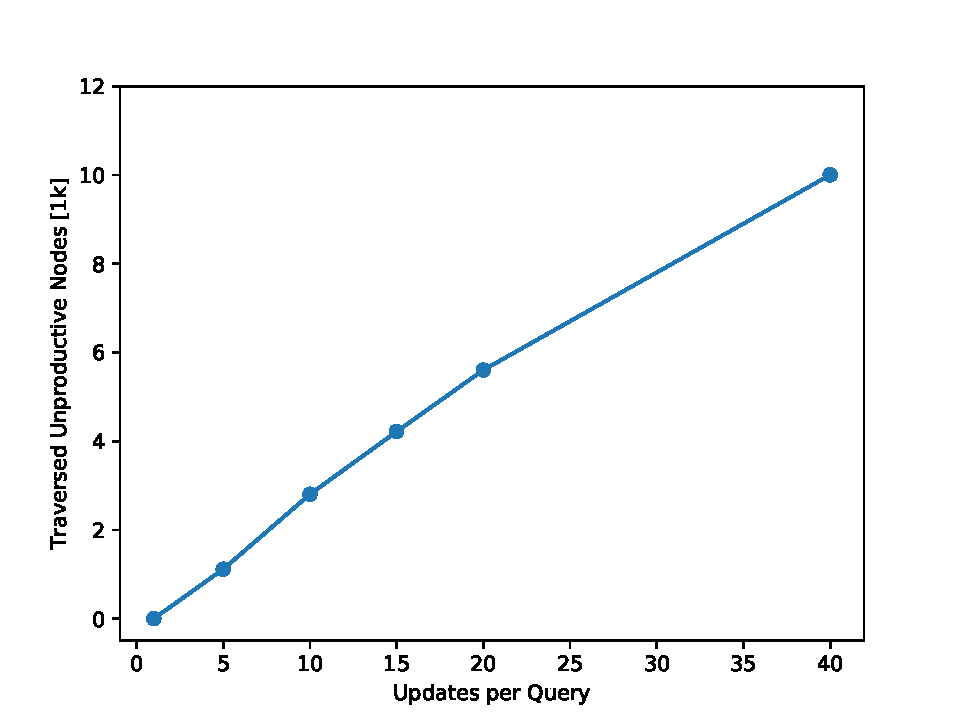
\includegraphics[width=8cm]{upt_unprod_nodes_synthetic}
    \label{fig:upt_unprod_nodes_synthetic}
  \end{subfigure}
  \begin{subfigure}{0.49\linewidth}
    \centering
    \caption{Real-World}
    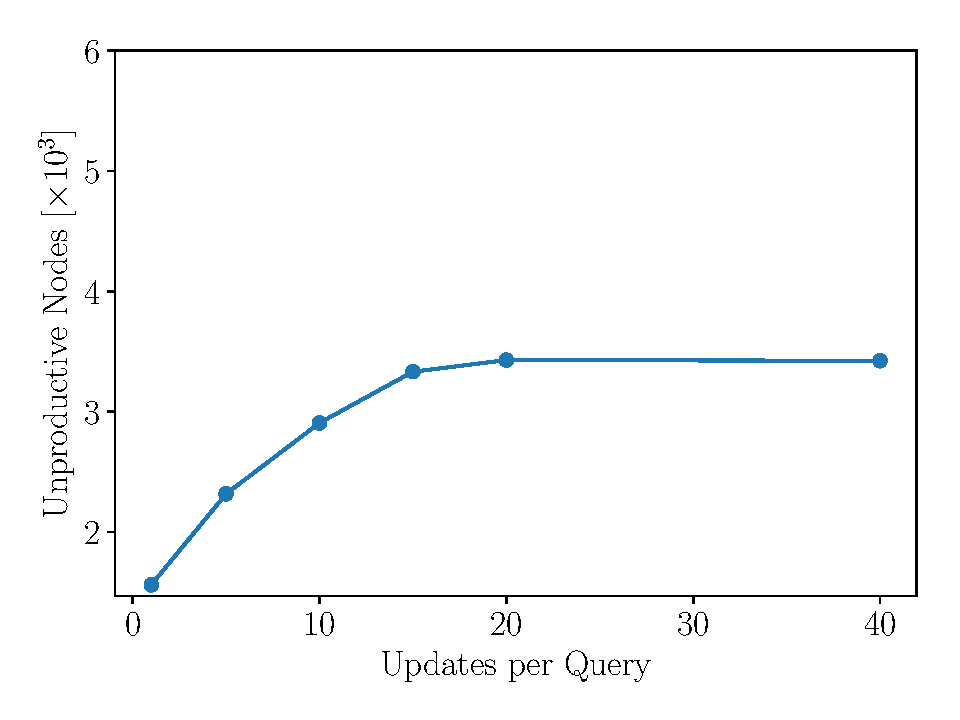
\includegraphics[width=8cm]{upt_unprod_nodes_real}
    \label{fig:upt_unprod_nodes_real}
  \end{subfigure}
  \vspace{-0.5cm}
  \caption{Traversed Unproductive Nodes over updates per query.}
\end{figure}

In addition, the increase we observe is sublinear. As mentioned in the previous Sections,
since the number of unproductive nodes has an upper bound set by the number
of content nodes, the function must converge towards this upper bound.

\subsection{Garbage Collection}

\label{sec:gc-experiment}

Our next experiment evaluates Oak's query performance under periodic Garbage Collection.
We record the average query runtime and the number of volatile and unproductive 
index nodes during query execution while having periodic GC enabled.

\begin{figure}[h]
  \centering
  \begin{subfigure}{0.49\linewidth}
    \centering
    \caption{Synthetic}
    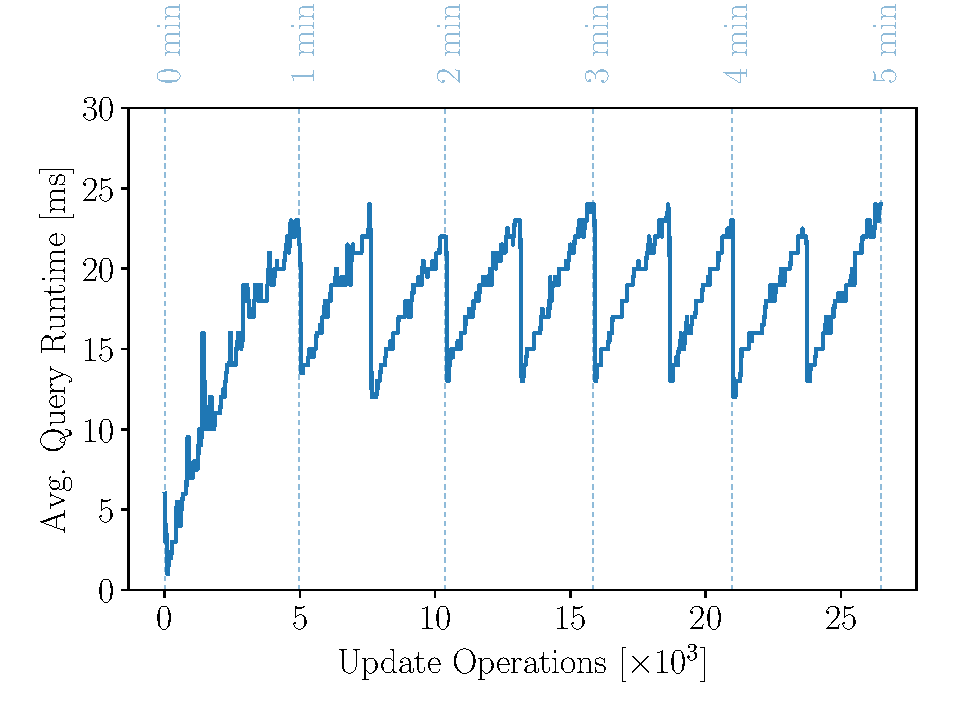
\includegraphics[width=8cm]{query_runtime_GC_synthetic}
    \label{fig:query_runtime_GC_synthetic}
  \end{subfigure}
  \begin{subfigure}{0.49\linewidth}
    \centering
    \caption{Real-World}
    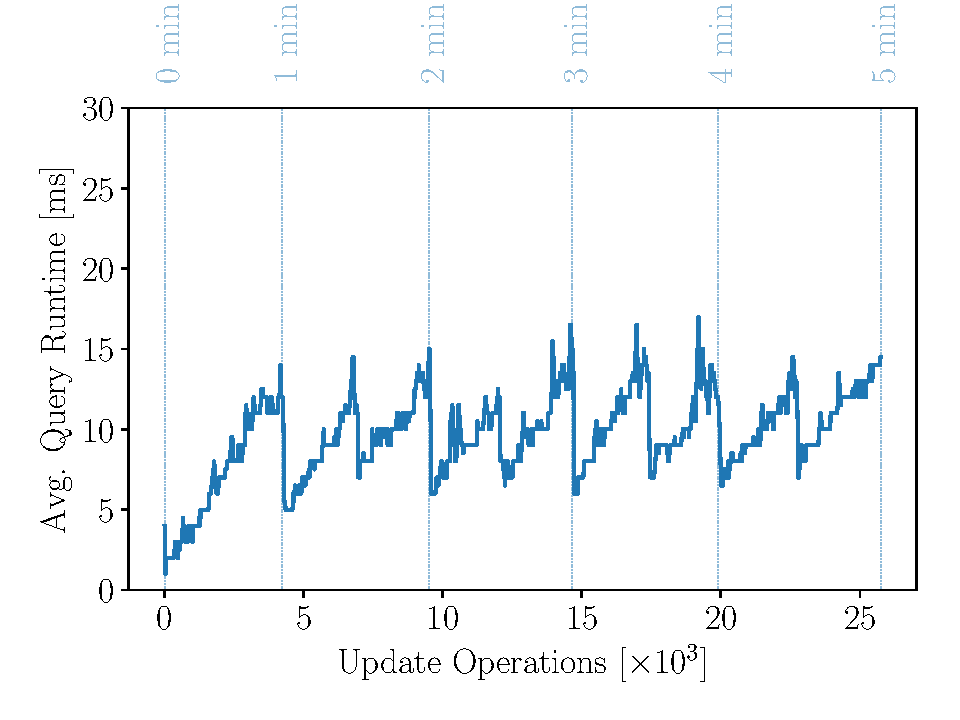
\includegraphics[width=8cm]{query_runtime_GC_real}
    \label{fig:query_runtime_GC_real}
  \end{subfigure}
  \vspace{-0.5cm}
  \caption{Query Runtime over update operations, periodic GC enabled.}
\end{figure}

\Cref{fig:query_runtime_GC_synthetic,fig:query_runtime_GC_real} show the
resulting decrease in query runtime when applying periodic GC on Oak. The
garbage collector is run every 30 seconds. We observe the query runtime
increase during the first minute of the simulation. 
When GC is run for the first time (at 30 seconds), it does not encounter
any unproducitve nodes because with $L=30s$ no volatile node has. Afterwards, every succeeding GC encounters
and prunes unproductive nodes. The pruned nodes are made visible by the
sawtooth pattern depicted in the Figure. 
Each drop in query runtime reflects the speedup caused by cleaning unproductive
nodes. The query runtime oscillates between
20 and 30 milliseconds with a mean of 25 milliseconds on the synthetic dataset.
The real world's query runtime oscillates between 8 and 18 milliseconds with a mean
value of 13 milliseconds.

We also observe that queries executed on the real-world dataset are faster,
on average. We will see later that the synthetic dataset has more index
nodes compared to the real-world dataset. The query executor has to traverse
more nodes under the synthetic dataset, hence the query runtime increases.

\begin{figure}[ht]
  \centering
  \begin{subfigure}{0.49\linewidth}
    \centering
    \caption{Synthetic}
    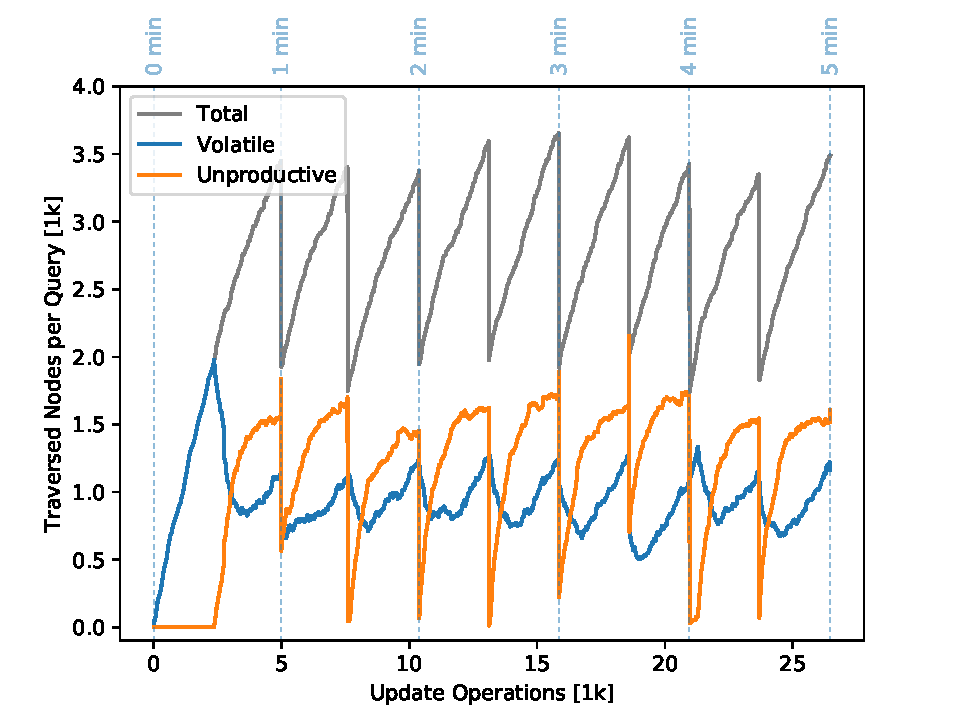
\includegraphics[width=8cm]{trav_nodes_GC_synthetic}
    \label{fig:trav_nodes_GC_synthetic}
  \end{subfigure}
  \begin{subfigure}{0.49\linewidth}
    \centering
    \caption{Real-World}
    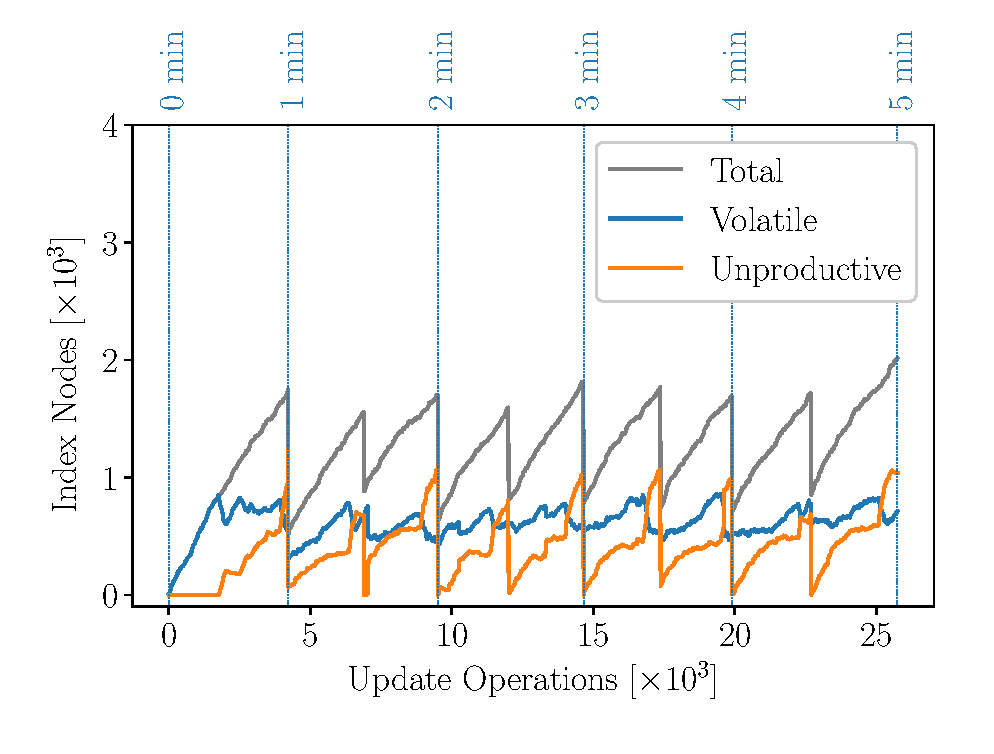
\includegraphics[width=8cm]{trav_nodes_GC_real}
    \label{fig:trav_nodes_GC_real}
  \end{subfigure}
  \vspace{-0.5cm}
  \caption{Index Nodes over update operations, periodic GC enabled.}
\end{figure}

\Cref{fig:trav_nodes_GC_synthetic,fig:trav_nodes_GC_real} visualize the index
structure during query execution with periodic GC. Unproductive
nodes increase until GC is run, after which they are completely removed again.
Observing the Figures, the number of unproductive nodes does not always reach zero.
That is because we use a moving median. The moving median removes outliers, and in
our case also points which had zero unproductive nodes.

The traversed volatile nodes have a cycloid pattern, as seen and explained in
\Cref{fig:trav_nodes_synthetic,fig:trav_nodes_real}.
In contrast to \Cref{fig:trav_nodes_synthetic,fig:trav_nodes_real}, 
we do not see the number of volatile nodes
having a downward trend anymore from the 30 second mark.
Instead in \Cref{fig:trav_nodes_GC_synthetic,fig:trav_nodes_GC_real}, 
the number of unproductive nodes oscillates around a constant throughout the experiment. 
Since the likelihood of node becoming volatile remains constant, there is no
increase or decrease in volatile nodes, on average.

Comparing the synthetic dataset to the real-world dataset, we observe another phenomenon.
The gap between traversed volatile and total traversed nodes is significantly bigger
in the synthetic dataset. In other words, the percentage of volatile index nodes
is higher in the real-world dataset. We believe that non-volatile
ancestors of volatile nodes account for the gap. 
We believe ancestors of volatile nodes are more likely to become volatile in
sparser subtrees. Sparse subtrees form long linked lists of nodes. If a leaf node
in such a linked list becomes volatile, so do its ancestors, since they are also
updated when the leaf node is added/removed. The more sparse a subtree is, the longer
the linked lists become.
Since the real-world dataset is sparser than the synthetic dataset (\Cref{sec:datasets}),
the percentage of volatile nodes is higher compared to the synthetic dataset.
%If the leaf node in such a chain is updated, each 
%ancestor in the chain is also added or removed, given they are not volatile. In that scenario,
%when the leaf node becomes volatile, its ancestors inside the chain most likely also become
%volatile, since they were added or removed every time the leaf node did. It is more likely
%for an ancestor to become volatile in the real-world dataset due to the long chains, hence
%the higher ratio of traversed volatile over total traversed index nodes.

\subsubsection{GC Period $T$}

\label{sec:periodicity}

In this section we discuss the performance impact of GC period $T$. Oak can run
GC arbitrary many times. Given our setup, we would like to find out what the
optimal period of GC is. We run GC under varying period and compare
the results.

We expect the number of unproductive nodes to decrease as we run GC more often,
i.e., $T$ decreases. GC uses system resources and if GC is run too often,
we might decrease the query performance because the system is busy garbage
collecting instead of executing queries.

For the following experiments, we allocate only a single virtual core to the
virtual machine in order to disable parallel computation. Since GC is run
on a different thread than the query executor, we have to ensure that GC's
thread steals CPU time from the query executor so that we can demonstrate
GC's cost.

\begin{figure}[ht]
  \centering
  \begin{subfigure}{0.49\linewidth}
    \centering
    \caption{Synthetic}
    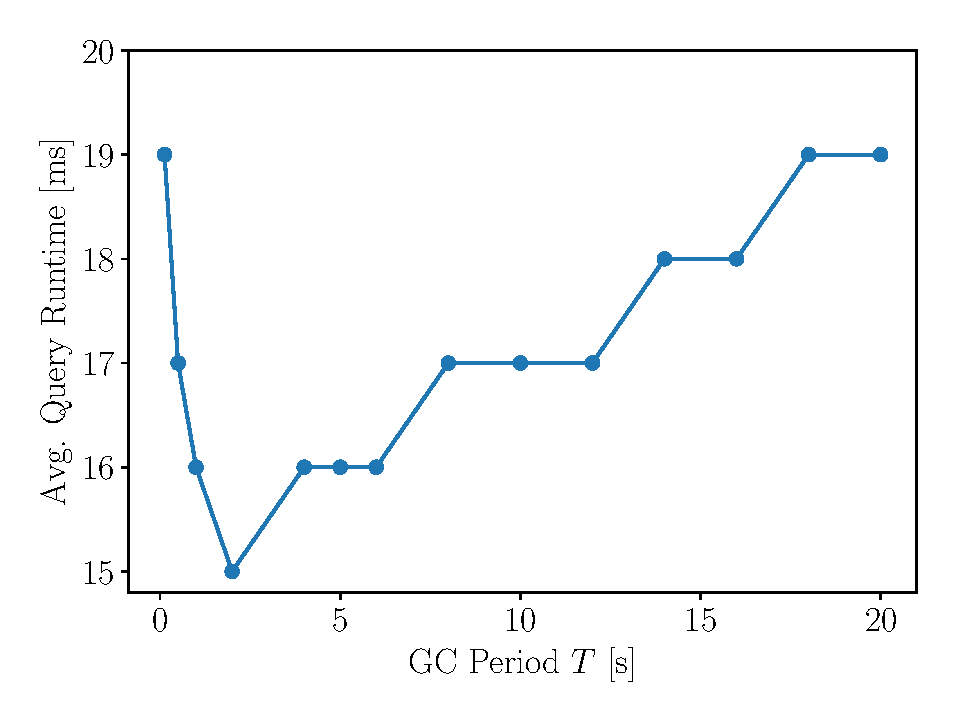
\includegraphics[width=8cm]{periodicity_query_runtime_synthetic}
    \label{fig:period_runtime_synthetic}
  \end{subfigure}
  \begin{subfigure}{0.49\linewidth}
    \centering
    \caption{Real-World}
    \includegraphics[width=8cm]{periodicity_query_runtime_real}
    \label{fig:period_runtime_real}
  \end{subfigure}
  \vspace{-0.5cm}
  \caption{Avg. Query Runtime over GC Period $T$.}
\end{figure}

%\begin{figure}[h]
  %\centering
  %\begin{subfigure}{0.49\linewidth}
    %\centering
    %Synthetic
  %\end{subfigure}
  %\begin{subfigure}{0.49\linewidth}
    %\centering
    %Real-World
  %\end{subfigure}
  %\begin{subfigure}{0.49\linewidth}
    %\centering
    %\includegraphics[width=8cm]{query_runtime_periodicity_synthetic}
    %\caption{}
    %\label{fig:query_runtime_periodicity_synthetic}
  %\end{subfigure}
  %\begin{subfigure}{0.49\linewidth}
    %\centering
    %\includegraphics[width=8cm]{query_runtime_periodicity_real}
    %\caption{}
    %\label{fig:query_runtime_periodicity_real}
  %\end{subfigure}
  %\caption{Query Runtime over update operations with GC period $T \in \{5s,50s\}$ }
%\end{figure}

%\begin{figure}[h]
  %\centering
  %\begin{subfigure}{0.49\linewidth}
    %\centering
    %Synthetic
  %\end{subfigure}
  %\begin{subfigure}{0.49\linewidth}
    %\centering
    %Real-World
  %\end{subfigure}
  %\begin{subfigure}{0.49\linewidth}
    %\centering
    %\includegraphics[width=8cm]{periodicity_query_runtime_synthetic}
    %\caption{}
    %\label{fig:periodicity_query_runtime_synthetic}
  %\end{subfigure}
  %\begin{subfigure}{0.49\linewidth}
    %\centering
    %\includegraphics[width=8cm]{periodicity_query_runtime_real}
    %\caption{}
    %\label{fig:periodicity_query_runtime_real}
  %\end{subfigure}
%\caption{Query Runtime over GC period $T$}
%\end{figure}

\Cref{fig:period_runtime_synthetic,fig:period_runtime_real} 
show the average query runtime with respect to period $T$.
The optimal period $T^*$ seems to be in the interval $T^* \in [500ms,2000ms]$ for
both datasets. If $T < T^*$, GC starts stealing CPU time
from the query executor and queries take longer to process.
On the other hand, when $T > T^*$, the query runtime increases sublinearly because
the index fills up with unproductive nodes. We see a sublinear increase since
the index becomes more static over time, as explained previously.

\begin{figure}[h]
  \centering
  \begin{subfigure}{0.49\linewidth}
    \centering
    \caption{Synthetic}
    \includegraphics[width=8cm]{trav_unprod_nodes_periodicity_synthetic}
    \label{fig:trav_unprod_nodes_periodicity_synthetic}
  \end{subfigure}
  \begin{subfigure}{0.49\linewidth}
    \centering
    \caption{Real-World}
    \includegraphics[width=8cm]{trav_unprod_nodes_periodicity_real}
    \label{fig:trav_unprod_nodes_periodicity_real}
  \end{subfigure}
  \vspace{-0.5cm}
  \caption{Traversed Unproductive Nodes over update operations with GC period $T \in \{5s, 50s\}$.}
\end{figure}

Let us consider 
\Cref{fig:trav_unprod_nodes_periodicity_synthetic,fig:trav_unprod_nodes_periodicity_real}.
They show the number of traversed unproductive nodes for two different periods
$T \in \{5s,50s\}$, with respect to update operations. We clearly see that GC with
period $T = 5s$ has a smaller number of unproductive nodes over time, on average.

\begin{figure}[h]
  \centering
  \begin{subfigure}{0.49\linewidth}
    \centering
    \caption{Synthetic}
    \includegraphics[width=8cm]{periodicity_unprod_nodes_synthetic}
    \label{fig:periodicity_unprod_nodes_synthetic}
  \end{subfigure}
  \begin{subfigure}{0.49\linewidth}
    \centering
    \caption{Real-World}
    \includegraphics[width=8cm]{periodicity_unprod_nodes_real}
    \label{fig:periodicity_unprod_nodes_real}
  \end{subfigure}
  \vspace{-0.5cm}
  \caption{Traversed Unproductive Nodes over GC period $T$.}
\end{figure}

\Cref{fig:periodicity_unprod_nodes_synthetic,fig:periodicity_unprod_nodes_real}
depict the number of unproductive nodes with respect to $T$. We see that the
number of unproductive nodes increases sublinearly as $T$ increases.
The function converges because the index becomes more static over time, as
explained previously.

\subsection{Query-Time Pruning}

\label{sec:qtp-experiment}

In this section, we evaluate Oak's query performance under Query-Time
Pruning. We record the average query runtime and the number of volatile
and unproductive index nodes, similar to \Cref{sec:gc-experiment}.

\begin{figure}[h]
  \centering
  \begin{subfigure}{0.49\linewidth}
    \centering
    \caption{Synthetic}
    \includegraphics[width=8cm]{query_runtime_QTP_synthetic}
    \label{fig:query_runtime_QTP_synthetic}
  \end{subfigure}
  \begin{subfigure}{0.49\linewidth}
    \centering
    \caption{Real-World}
    \includegraphics[width=8cm]{query_runtime_QTP_real}
    \label{fig:query_runtime_QTP_real}
  \end{subfigure}
  \vspace{-0.5cm}
  \caption{Query Runtime over update operations, QTP enabled.}
\end{figure}

\begin{figure}[h]
  \centering
  \begin{subfigure}{0.49\linewidth}
    \centering
    \caption{Synthetic}
    \includegraphics[width=8cm]{trav_nodes_QTP_synthetic}
    \label{fig:trav_nodes_QTP_synthetic}
  \end{subfigure}
  \begin{subfigure}{0.49\linewidth}
    \centering
    \caption{Real-World}
    \includegraphics[width=8cm]{trav_nodes_QTP_real}
    \label{fig:trav_nodes_QTP_real}
  \end{subfigure}
  \vspace{-0.5cm}
  \caption{Index Nodes over update operations, QTP enabled.}
\end{figure}

\Cref{fig:query_runtime_QTP_synthetic,fig:query_runtime_QTP_real} depict the
resulting decrease in query runtime when applying QTP on Oak. We see the runtime
rise during the first 30 seconds and then see the runtime remain stable.
We believe that traversing volatile nodes dominates query runtime. 

\Cref{fig:trav_nodes_QTP_synthetic,fig:trav_nodes_QTP_real} show the composition
of the index with QTP enabled during query execution. We observe the number of
unproductive nodes to be close to 0 throughout the entire simulation. This is
because the index is continuously cleaned by QTP. As long as query execution is
continuous, so is our index cleaning. Since after ten updates we always query the root content
node in our experiment, we clean the whole index subtree from unproductive nodes.
QTP also cleans unproductive nodes the moment they spawn. In contrast, periodic GC
cleans these unproductive nodes 30 seconds after they spawn, in our experiment.

As seen previously with GC (\Cref{sec:gc-experiment}), 
we also observe a bigger gap between volatile and total
index nodes in the synthetic dataset compared to the real-world one due to
more non-volatile ancestors of volatile nodes.

The workload during the experiment always queries the content subtree root node. 
It still remains open how QTP affects performance when the query filter changes 
more often and frequent queries do not benefit from QTP anymore.

It is also worth mentioning what the performance penalty of QTP is when
there are no unproductive nodes.
The performance penalty occurs when the query executor has to compute if each
node is volatile in order to detect unproductive nodes.

%\Cref{fig:query_runtime_qtp_cost_synthetic,fig:query_runtime_qtp_cost_real}
%compare the average query runtime over update operations, with QTP and without.
%The experiments last for 5 minutes and the volatility threshold is $\tau = 0$.
%Since $\tau = 0$, there are no unproductive nodes during the experiments.
%We observe that queries with QTP tend to require 60\% more time on average than
%without QTP and therefore queries without QTP perform better, when there are
%no unproductive nodes. Obviously, once we encounter unproductive nodes, queries
%with QTP perform better, as shown in \Cref{fig:query_runtime_QTP_synthetic,fig:query_runtime_QTP_real}.

\begin{figure}[H]
  \centering
  \begin{subfigure}{0.49\linewidth}
    \centering
    \includegraphics[width=8cm]{qtp_cost_synthetic}
  \end{subfigure}
  \begin{subfigure}{0.49\linewidth}
    \centering
    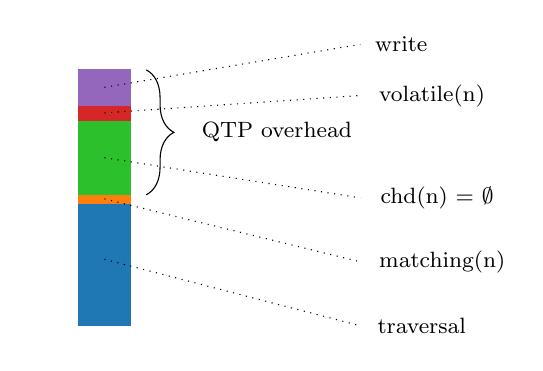
\begin{tikzpicture}[scale=0.65]
        \fill[transparent] (-1,0) rectangle (0,5.5);
        \filldraw[color=C0] (0,0) rectangle (1,2.40);
        \filldraw[color=C1] (0,2.40) rectangle (1,2.56);
        \filldraw[color=C2] (0,2.56) rectangle (1,4.01);
        \filldraw[color=C3] (0,4.01) rectangle (1,4.31);
        \filldraw[color=C4] (0,4.31) rectangle (1,5);
        \fill[transparent] (0,5) rectangle (1,5.5);

        \draw[dotted] (0.5,1.3) -- (5.5,0);
        \node[align=left] at (6.7,0) {\footnotesize traversal};

        \draw[dotted] (0.5,2.48) -- (5.5,1.25);
        \node[align=left] at (7.1,1.25) {\footnotesize matching(n)};
        \draw[dotted] (0.5,3.285) -- (5.5,2.5);
        \node[align=left] at (7,2.5) {\footnotesize chd(n) = $\emptyset$};
        \draw[dotted] (0.5,4.16) -- (5.5,4.5);
        \node[align=left] at (6.9,4.5) {\footnotesize volatile(n)};
        \draw[dotted] (0.5,4.66) -- (5.5,5.5);
        \node[align=left] at (6.3,5.5) {\footnotesize write};
       \draw [decorate,decoration={brace,amplitude=10pt,mirror,raise=4pt},yshift=0pt]
       (1.1,2.56) -- (1.1,5.0) node [black,midway,xshift=1.8cm] {\footnotesize
       QTP overhead};
   \end{tikzpicture}
  \end{subfigure}
  \caption[QTP overhead]{The overhead of various steps during QTP
  are highlighted with different colors. A 20ms query spends on average 10ms 
  (50\%) traversing, 0.5ms (2.5\%) checking the match property, 6ms (30\%) checking
  for children, 0.5ms (2.5\%) checking for volatility and 3ms (15\%) writing. QTP
  added a 9.5ms (+90\%) overhead.
  }
    \label{fig:qtp-overhead}
\end{figure}

\Cref{fig:qtp-overhead} depicts a cost breakdown of a QTP query. A 20ms query
spends on average 10ms (50\%) traversing the index subtree, 0.5ms (2.5\%) checking
the match property of visited nodes, 6ms (30\%) checking if the visited nodes
have children, 0.5ms (2.5\%) checking if the visited nodes are volatile and 3ms
(15\%) writing, that is pruning unproductive nodes and commiting the transaction.

QTP added a 9.5ms overhead to a 11.5ms query, which corresponds to an additional 90\%
runtime. Please note that a normal query would only take 11.5ms if there are no
unproductive index nodes. The main overhead added by QTP is checking if the visited 
nodes have children. Checking the match property and checking if a node is volatile, 
are cheap operations because Oak caches node properties internally.

\subsection{Comparison}

\label{sec:comparison}

\subsection{Summary}

\label{sec:summary}

\Cref{sec:experimental-evaluation} focused on the experimental evaluation.
We first conducted a series of experiments to test parameters that
impact the production of unproductive nodes. Later on we benchmarked the
query performance of periodic Garbage Collection and Query-Time pruning.

In \Cref{sec:threshold}, we tested different volatility thresholds $\tau$
and saw that a lower $\tau$ increases the number of unproductive nodes in
index subtree. $\tau$ and unproductive nodes share a power law relationship.

In \Cref{sec:sliding-window}, we investigated what the effect of the
sliding window length $L$ is on unproductive index nodes. The results
of the experiments suggest a linear relationship between $L$ and the
number of unproductive nodes, but we expect a sublinear increase if
the experiment is run longer.

\Cref{sec:skew} focuses on the workload's skew $s$. We saw how the
number of unproductive nodes drops rapidly for high values of $s$.
The hotspot gets smaller and therefore we observe less unproductive nodes.

In \Cref{sec:update-query-ratio}, we shift our attention to the ratio between
queries and updates. We see that executing more updates with respect
to the queries, the number of unproductive index nodes increases sublinearly.

\Cref{sec:gc-experiment,sec:periodicity} benchmark periodic GC. We showed
that queries are executed faster due to less unproductive index nodes.
Running GC more often reduces the number of unproductive nodes in the index,
but running GC too often steals CPU resources from query execution and
adds a performance penalty to the queries. The system is busy garbabe
collecting instead of answering queries.

In \Cref{sec:qtp-experiment}, we test QTP, the second approach we
proposed for cleaning unproductive nodes from the index. We saw that
the number of unproductive nodes was near zero throughout the entire
five-minute experiment. That was the case, because queries under
QTP were cleaning the index continuoysly. We later analyzed the
cost structure of a query under QTP. The average query runtime increased
from 11.5ms to 20ms. The main overhead of QTP is checking if the visited
nodes have children, which is done to determine if nodes are unproductive.

\newpage\null\thispagestyle{empty}\newpage

\section{Conclusion}

We proposed two algorithms to detect and prune unproductive nodes in hotspots of a
hierarchical index. Unproductive nodes are useless since they do not contain any data.
By pruning these unproductive nodes, we are able to improve the
index query performance since we only encounter index nodes that do yield a
query match, are volatile, or are an ancestor of such a node.
Additionally, we free storage space that was previously allocated to unproductive nodes.

The first approach is to periodically apply garbage collection (GC) on WAPI. Doing so
requires us to explicitly traverse the index subtree thus introducing a performance penalty,
but we are able to prune all unproductive nodes from the index.
The second approach is to prune unproductive nodes during query execution (QTP). Doing so we
don't have to explicitly traverse the index, but we add a small overhead on query execution
because we have to compute each visited node's volatility.
Additionally, we only prune unproductive nodes from subtrees which are being queried.
We extend WAPI by implementing periodic GC and QTP in Apache Jackrabbit Oak
and our evaluation shows that we significantly decrease the query runtime of WAPI.

Our experimental evaluation also showed that volatility threshold $\tau$, sliding
window of length $L$, the update to query ratio and skew $s$, impact the number
of volatile nodes in the index subtree, which later on most likely become
unproductive and slow down queries.

It is still open how concurrency control affects the performance of the two mentioned
algorithms. We believe QTP will take a bigger permormance hit in comparison to GC, since
QTP continuously prunes and updates the index causing more index conflicts than
GC with its periodic updates. Furthemore, we did not investigate what the benefits and caveats
are of running both periodic GC and QTP simultaneously on the database system.

\newpage

\bibliographystyle{abbrv}
\bibliography{thesis}

\newpage

\section{Appendix}

\begin{figure}[H]
  \centering
  \small
  \begin{framed}
\begin{minted}{java}
/**
 * Returns an iterable which lazily traverses a subtree rooted at root
 * in postorder.
 *
 * @param root: Root node of subtree we apply traversal on
 * @returns: Iterable for postorder tree walk
 */
Iterable<Tree> postOrder(Tree root) {
    return () -> {
        /* Stacks */
        Deque<Tree> s1 = new LinkedList();
        Deque<Tree> s2 = new LinkedList();
        s1.push(root);
        return new Iterator<Tree>() {
            @Override
            public boolean hasNext() {
                return s1.size() > 0 || s2.size() > 0;
            }
            @Override
            public Tree next() {
                while (s1.size() > 0 && (
                    s2.size() == 0 ||
                        isAncestor(
                            s2.peek().getPath(),
                            s1.peek().getPath()
                        )
                )) {
                    Tree n = s1.pop();
                    s2.push(n);
                    for (Tree child : n.getChildren()) {
                        s1.push(child);
                    }
                }
                return s2.pop();
            }          
        };
    };
}
\end{minted}
  \end{framed}
  \caption{\texttt{postOrder()} implementation in Java.}
  \label{fig:java_postorder}
\end{figure}

\begin{figure}[h]
  \begin{framed}
\begin{minted}{java}
/**
 * Higher order function, applies func to each element of iterable.
 *
 * @param func: The function to apply on each element of iterable
 * @param iterable: The iterable func is applied on
 * @returns: Resulting elements from applying func
 */
Iterable<R> map(Function<T,R> func, Iterable<T> iterable) {
    return () -> {
        Iterator<T> iterator = iterable.iterator();
        return new Iterator<R>() {
            @Override
            public boolean hasNext() {
                return iterator.hasNext();
            }
            @Override
            public R next() {
                return func.apply(iterator.next());
            }
        };
    };
}
\end{minted}
  \end{framed}
  \caption{\texttt{map()} implementation in Java.}
  \label{fig:java_map}
\end{figure}

\begin{figure}[h]
  \begin{framed}
\begin{minted}{java}
/**
 * Higher order function that removes all elements from an iterable
 * not satisfying the predicate.
 *
 * @param predicate: The predicate that tests elements
 * @param iterable: The iterable whose members are tested against
 * @returns: An iterable with members satisfying the predicate
 */
Iterable<T> filter(Predicate<T> predicate, Iterable<T> iterable) {
    return () -> {
        Iterator<T> iterator = iterable.iterator();
        T n = null;
        return new Iterator<T>() {
            @Override
            public boolean hasNext() {
                nextIfNeeded();
                return n != null; 
            }
            @Override
            public T next() {
                nextIfNeeded();
                T tmp = n;
                n = null;
                return tmp;
            }
            @Override
            private void nextIfNeeded() {
                while (n == null && iterator.hasNext()) {
                    T candidate = iterator.next();
                    if (predicate.test(candidate)) {
                        n = candidate;
                    }
                }
            }
        };
    };
}
\end{minted}
  \end{framed}
  \caption{\texttt{filter()} implementation in Java.}
  \label{fig:java_filter}
\end{figure}

\end{document}
